\chapter{进入保护模式} \label{CHpm}

前面我们看到,通过一些很简单的代码,我们做到了启动一个微型系统,加载文件系统中的文件进入内存并运行的功能。应该注意的是,在前面的代码中我们使用的内存空间都很小。我们看一下~boot.bin~和~LOADER.BIN~的大小就能感觉出来(当然,可执行文件小未必使用内存空间小,但是这两个文件也太小了~\smiley)。

\begin{Command}
$ ls -l boot.bin LOADER.BIN 
-rwxr-xr-x 1 solrex solrex 512 2008-04-26 16:34 boot.bin
-rwxr-xr-x 1 solrex solrex  15 2008-04-26 16:34 LOADER.BIN
\end{Command}

boot.bin~是~512~个字节(其中还有我们填充的内容,实际指令只有~480~个字节),而~LOADER.BIN~更过分,只有~15~个字节大小。可想而知这两个文件在内存中能使用多大的空间吧。如果读者有些汇编语言经验的话,就会发现我们在前面的程序中使用的存储器寻址都是在实模式下进行的,即:由段寄存器(cs,~ds:~16-bit)配合段内偏移地址(16-bit)来定位一个实际的~20-bit~物理地址,所以我们前面的程序最多支持~$2^{20} = 2^{10}*2^{10} = 1024*1024$ bytes = 1MB~的寻址空间。

哇,~1MB~不小了,我们的操作系统加一起连~1KB~都用不到,~1MB~寻址空间足够了。但是需要考虑到的一点是,就拿我们现在用的~1.44MB的(已经被淘汰的)软盘标准来说,如果软盘上某个文件超过~1MB~,我们的操作系统就没办法处理了。那么如果以后把操作系统安装到硬盘上之后呢?我们就没办法处理稍微大一点的文件了。

所以我们要从最原始的~Intel 8086/8088 CPU~的实模式中跳出来,进入~Intel 80286~之后系列~CPU~给我们提供的保护模式。这还将为我们带来其它更多的好处,具体内容请继续往下读。

\section{实模式和保护模式}

\BOXED{0.9\textwidth}{
\danger\\ 如果您需要更详细的知识,也许您更愿意去读 Intel 的手册,本节内容主要集中在:\href{http://download.intel.com/design/processor/manuals/253668.pdf}{Intel\textregistered~64 and IA-32 Architectures Software Developer's Manual, Volume 3A: System Programming Guide}, 第~2~章和第~3~章.\enddanger
}

\subsection{一段历史}

Intel~公司在~1978~年发布了一款~16~位字长~CPU: 8086~,最高主频~5 MHz$\sim$10 MHz~,集成了~29,000~个晶体管,这款在今天感觉像玩具一样的~CPU~却是奠定今天~Intel PC~芯片市场地位的最重要的产品之一。虽然它的后继者~8088~,加强版的~8086~(增加了一个~8~比特的外部总线)才是事实上的~IBM~兼容机(PC,个人电脑)雏形的核心,但人们仍然习惯于用~8086~作为厂商标志代表~Intel~。

因为受到字长(16~位)的限制,如果仅仅使用单个寄存器寻址,~8086~仅仅能访问~64KB($2^{16}$)~的地址空间,这显然不能满足一般要求,而当时~1MB($2^{20}$)~对于一般的应用就比较足够了,所以~8086~使用了~20~位的地址线。

在~8086~刚发布的时候,没有“实模式”这个说法,因为当时的~Intel CPU~只有一种模式。在~Intel~以后的发布中,~80286~引入了“保护模式”寻址方式,将~CPU~的寻址范围扩大到~16($2^{24}$) MB~,但是~80286~仍然是一款~16~位~CPU~,这就限制了它的广泛应用。但是“实模式”这个说法,就从~80286~开始了。

接下来的发展就更快了,1985~年发布的~i386~首先让~PC CPU~进入了~32~位时代,由此而带来的好处显而易见,寻址能力大大增强,但是多任务处理和虚拟存储器的需求仍然推动着~i386~向更完善的保护模式发展。下面我们来了解一下“实模式”和“保护模式”的具体涵义。

\subsection{实模式}

实模式(real mode),有时候也被成为实地址模式(real address mode)或者兼容模式(compatibility mode)是~Intel 8086 CPU~以及以其为基础发展起来的~x86~兼容~CPU~采用的一种操作模式。其主要的特点有:20~比特的分段访问的内存地址空间(即~1~MB~的寻址能力);程序可直接访问~BIOS~中断和外设;硬件层不支持任何内存保护或者多任务处理。~80286~之后所有~x86 CPU~在加电自举时都是首先进入实模式;~80186~以及之前的~CPU~只有一种操作模式,相当于实模式。

\subsection{保护模式}

保护模式(protected mode),有时候也被成为保护的虚拟地址模式(protected virtual address mode),也是一种~x86~兼容~CPU~的工作模式。保护模式为系统软件实现虚拟内存、分页机制、安全的多任务处理的功能支持,还有其它为操作系统提供的对应用程序的控制功能支持,比如:特权级、实模式应用程序兼容、虚拟~8086~模式。

\subsection{实模式和保护模式的寻址模式}

前面提到过,实模式下的地址线是~20~位的,所以实模式下的寻址模式使用分段方式来解决~16~位字长机器提供~20~位地址空间的问题。这个分段方法需要程序员在编制程序的过程中将存储器划分成段,每个段内的地址空间是线性增长的,最大可达~64K($2^16$),这样段內地址就可以使用~16~位表示。段基址(~20-bit~)的最低~4~位必须是~0~,这样段基址就可以使用~16~位段地址来表示,需要时将段地址左移~4~位就得到段起始地址。除了便于寻址之外,分段还有一个好处,就是将程序的代码段、数据段和堆栈段等隔离开,避免相互之间产生干扰。

当计算某个单元的物理地址时,比如汇编语言中的一个~Label~,就通过段地址(~16-bit~)左移~4~位得到段基址(~20-bit~),再加上该单元(~Label~)的段內偏移量(~16-bit~)来得到其物理地址(~20-bit~),如图~\ref{rm_addr}~所示。

\begin{figure*}[!t]
\centerline{\subfloat[实模式寻址模型]{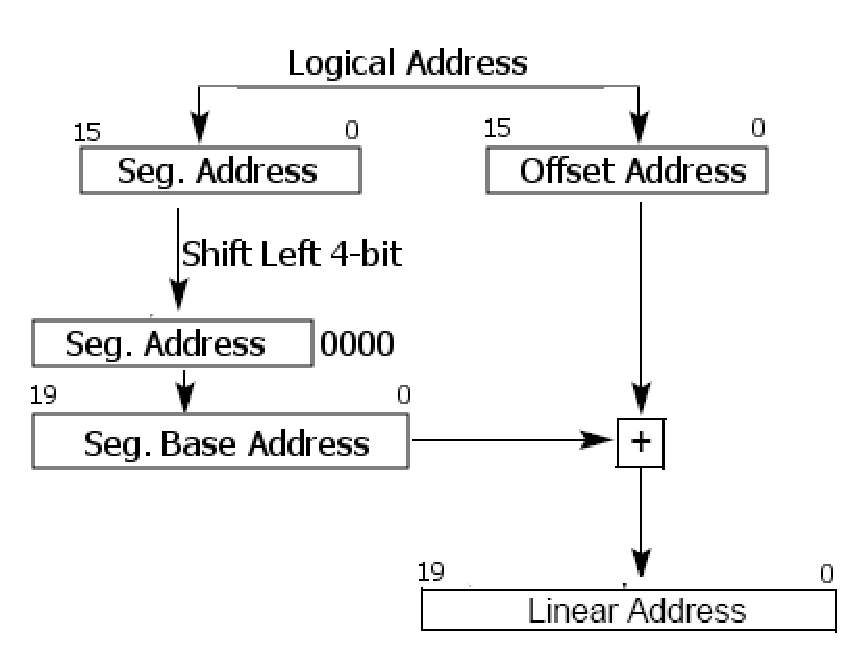
\includegraphics[width=.48\textwidth,keepaspectratio]{rm_addr}%
\label{rm_addr}}
\hfil
\subfloat[保护模式寻址模型]{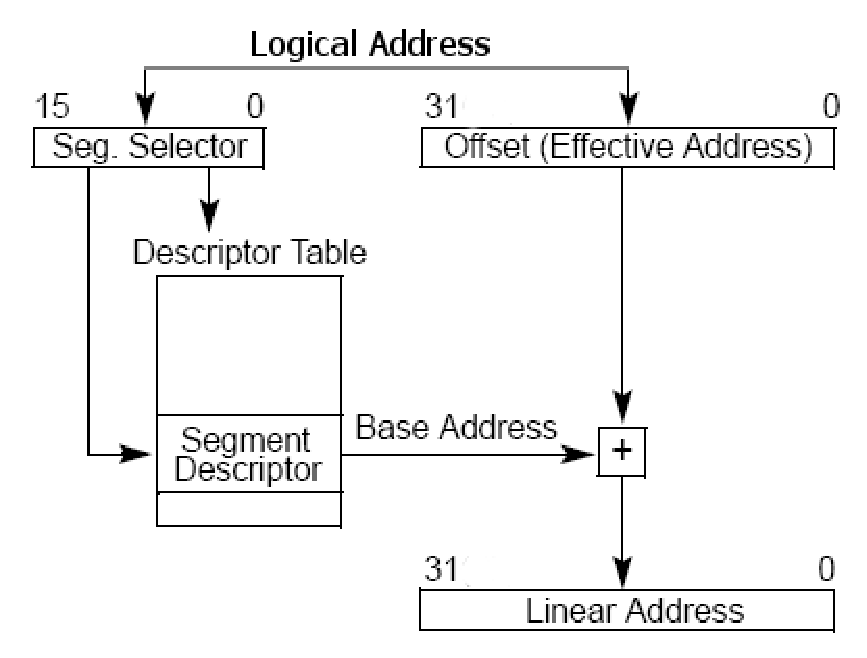
\includegraphics[width=.48\textwidth,keepaspectratio]{protected_seg}%
\label{protected_seg}}}
\caption{实模式与保护模式寻址模型比较}
\label{real_vs_pro}
\end{figure*}

一般情况下,段地址会被放在四个段寄存器中,即:代码段~CS,数据段~DS,堆栈段~SS~和附加段~ES~寄存器。这样在加载数据或者控制程序运行的时候,只需要一个偏移量参数,CPU~会自动用对应段的起始地址加上偏移量参数来得到需要的地址。(后继~CPU~又加上了两个段寄存器~FS~和~GS~,不过使用方式是基本一样的。)

由此可见,实模式的寻址模式是很简单的,就是用两个~16~位逻辑地址(段地址:偏移地址)组合成一个~20~位物理地址,而保护模式的寻址方式就要稍微复杂一点了。

\BOXED{0.9\textwidth}{
Intel~的~CPU~在保护模式下是可以选择打开分页机制的,但为了简单起见,我们先不开启分页机制,所以下面的讲解针对只有分段机制的保护模式展开。
}

在保护模式下,每个单元的物理地址仍然是由逻辑地址表示,但是这个逻辑地址不再由(段地址:偏移地址)组成了,而是由(段选择子:偏移地址)表示。这里的偏移地址也变成了~32~位的,所以段空间也比实模式下大得多。偏移地址的意思和实模式下并没有本质不同,但段地址的计算就要复杂一些了,如图~\ref{protected_seg}~所示。段基址(Segment Base Address)被存放在段描述符(Segment Descriptor)中,GDT(Global Descriptor Table,全局段选择子表)是保存着所有段选择子的信息,段选择子(Segment Selector)是一个指向某个段选择子的索引。

如图~\ref{protected_seg}~所示,当我们计算某个单元的物理地址时,只需要给出(段选择子:偏移地址),CPU~会从~GDT~中按照段选择子找到对应的段描述符,从段描述符中找出段基址,将段基址加上偏移量,就得到了该单元的物理地址。

\section{与保护模式初次会面}

介绍完了保护模式和实模式的不同,下面我们就尝试一下进入保护模式吧。在上一章我们已经实现了用启动扇区加载引导文件,所以这里我们就不用再去管启动扇区的事情了,下面的修改均在~loader.S~中进行。上一章的~loader.S~仅仅实现在屏幕的上方中间打印了一个~\code{L}~,下面我们的~loader.S~要进入保护模式来打印一些新东西。

首先,我们来理清一下应该如何进入保护模式:

\begin{enumerate}
  \item 我们需要一个~GDT。由于保护模式的寻址方式是基于~GDT~的,我们得自己写一个~GDT~数据结构并将其载入到系统中。
  \item 我们需要为进入保护模式作准备。由于保护模式和实模式运行方式不同,在进入保护模式之前,我们需要一些准备工作。
  \item 我们需要一段能在保护模式下运行的代码 demo,以提示我们成功进入了保护模式。
\end{enumerate}

下面我们就来一步步完成我们的第一个保护模式~loader~。

\subsection{GDT~数据结构}

要写~GDT,首先得了解~GDT~的数据结构。GDT~实际上只是一个存储段描述符的线性表(可以理解成一个段描述符数组),对它的要求是其第一个段描述符置为空,因为处理机不会去处理第一个段描述符,所以理解~GDT~的数据结构难点主要在于理解段描述符的数据结构。

段描述符主要用来为处理机提供段位址,段访问控制和状态信息。图~\ref{seg_desc}~显示了一个基本的段描述符结构:

\FIG{段描述符}{seg_desc}{.9\textwidth}

看到上面那么多内容,是不是感觉有点儿恐怖啊!其实简单的来看,我们现在最关注的是段基址,就是图~\ref{seg_desc}~中标记为~Base~的部分。可以看到,段基址在段描述符中被分割为三段存储,分别是:Base 31:24, Base 23:16, Base Address 15:0,把这三段拼起来,我们就得到了一个~32~位的段基址。

有了段基址,就需要有一个界限来避免程序跑丢发生段错误,这个界限就是图~\ref{seg_desc}~中标记为~Limit~的部分,将~Seg. Limit 19:16~和~Segment Limit 15:0~拼起来我们就得到了一个~20~位的段界限,这个界限就是应该是段需要的长度了。

下面还要说的就是那个~D/B Flag~,D/B~代表~Default Operation Size~,0~代表~16~位的段,1~代表~32~位的段。为了充分利用~CPU~,我们当然要设置为~32~位模式了。剩下那些乱七八糟的~Flag~呢,无非就是提供段的属性(代码段还是数据段?只读还是读写?),我们将在第~\ref{CHpm_desattr}~节为大家详细介绍。

这些东西那么乱,难道要每次一点儿一点儿地计算吗?放心,程序员自有办法,请看下面的程序:

\VerbatimInput[fontfamily=tt,fontsize=\footnotesize,frame=lines, framerule=0.4mm, numbers=left, numbersep=3pt, tabsize=2, firstline=56, lastline=70]{../src/chapter3/1/pm.h}
\codecaption{自动生成段描述符的宏定义(节自 chapter3/1/pm.h)}\label{CHpm_descm}

图~\ref{CHpm_descm}~中所示,就是自动生成段描述符的汇编宏定义。我们只需要给宏~Descriptor~三个参数:Base(段基址), Limit(段界限[段长度]), Attr(段属性),Descriptor~就会自动将三者展开放到段描述符中对应的位置。看看我们在程序中怎么使用这个宏:

\VerbatimInput[fontfamily=tt,fontsize=\footnotesize,frame=lines, framerule=0.4mm, numbers=left, numbersep=3pt, tabsize=2, firstline=21, lastline=26]{../src/chapter3/1/loader.S}
\codecaption{自动生成段描述符的宏使用示例(节自 chapter3/1/loader.S)}\label{CHpm_descmu}

图~\ref{CHpm_descmu}~中,就利用~Descriptor~宏生成了三个段描述符,形成了一个~GDT。注意到没有,第一个段描述符是空的(参数全为~0)。这里~LABEL\_DESC\_CODE32~的段基址为~0~是因为我们无法确定它的准确位置,它将在运行期被填入。

有人可能会产生疑问,段基址和段界限什么意思我们都知道了,那段属性怎么回事呢?~DA\_C, DA\_32, DA\_DRW~都是什么东西啊?是这样的,为了避免手动一个一个置段描述符中的~Flag~,我们预先定义了一些常用属性,用的时候只需要将这些属性加起来作为宏~Descriptor~的参数,就能将段描述符中的所有~flag~置上(记得~C~语言中~fopen~的参数吗?)。这些属性的定义如下(没必要细看,用的时候再找即可):

\VerbatimInput[fontfamily=tt,fontsize=\footnotesize,frame=lines, framerule=0.4mm, numbers=left, numbersep=3pt, tabsize=2, firstline=11, lastline=55]{../src/chapter3/1/pm.h}
\codecaption{预先设置的段属性(节自 chapter3/1/pm.h)}\label{CHpm_segattr}

\subsection{保护模式下的~demo}

为什么把这节提前到第~\ref{CHpm_secloadgdt}~节前讲呢?因为要写入~GDT~正确的段描述符,首先要知道段的信息,我们就得先准备好这个段:

\VerbatimInput[fontfamily=tt,fontsize=\footnotesize,frame=lines, framerule=0.4mm, numbers=left, numbersep=3pt, tabsize=2, firstline=82, lastline=99]{../src/chapter3/1/loader.S}
\codecaption{第一个在保护模式下运行的 demo(节自 chapter3/1/loader.S)}\label{CHpm_demo1}

其实这个段的作用很简单,通过操纵视频段数据,在屏幕中间打印一个红色的"P"(和我们前面使用~BIOS~中断来打印字符的方式有所不同)。

\subsection{加载~GDT} \label{CHpm_secloadgdt}

GDT~所需要的信息我们都知道了,GDT~表也通过图~\ref{CHpm_descmu}~中的代码实现了。那么,我们应该向~GDT~中填入缺少的信息,然后载入~GDT~了。将~GDT~载入处理机是用~\code{lgdt}~汇编指令实现的,但是~\code{lgdt}~指令需要存放~GDT~的基址和界限的指针作参数,所以我们还需要知道~GDT~的位置和~GDT~的界限:

\VerbatimInput[fontfamily=tt,fontsize=\footnotesize,frame=lines, framerule=0.4mm, numbers=left, numbersep=3pt, tabsize=2, firstline=17, lastline=63]{../src/chapter3/1/loader.S}
\codecaption{加载~GDT(节自 chapter3/1/loader.S)}\label{CHpm_loadgdt}

图~\ref{CHpm_loadgdt}~中~\code{GdtPtr}~所指,即为~GDT~的界限和基址所存放位置。某段描述符对应的~GDT~选择子,就是其段描述符相对于~GDT~基址的索引(在我们例子里~GDT~基址为~\code{LABEL\_GDT}~指向的位置)。这里需要注意的是,虽然我们在代码中写:

\begin{Command}
.set SelectorCode32, (LABEL_DESC_CODE32 - LABEL_GDT)
\end{Command}
但实际上段选择子在使用时需要右移~3~个位作为索引去寻找其对应的段描述符,段选择子的右侧~3~个位是为了标识~TI~和~RPL~的,如图~\ref{seg_selector}~所示,这点我们将在第~\ref{CHpm_ldt}~节和第~\ref{CHpm_desattr}~节中详细介绍。但是这里为什么能直接用地址相减得到段选择子呢?因为段描述符的大小是~8~个字节,用段描述符的地址相减的话,地址差的最右侧三个位就默认置~0~了。

在图~\ref{CHpm_loadgdt}~中所示的代码,主要干了两件事:第一,将图~\ref{CHpm_demo1}~所示~demo~的段基址放入~GDT~中对应的段描述符中;第二,将~GDT~的基址放到~\code{GdtPtr}~所指的数据结构中,并加载~\code{GdtPtr}~所指的数据结构到~GDTR~寄存器中(使用~\code{lgdt}~指令)。

\subsection{进入保护模式}

进入保护模式前,我们需要将中断关掉,因为保护模式下中断处理的机制和实模式是不一样的,不关掉中断可能带来麻烦。使用~\code{cli}~汇编指令可以清除所有中断~flag。

由于实模式下仅有~20~条地址线:A0, A1, \ldots, A19,所以当我们要进入保护模式时,需要打开~A20~地址线。打开~A20~地址线有至少三种方法,我们这里采用~IBM~使用的方法,通常被称为:“Fast A20 Gate”,即修改系统控制端口~92h~,因为其端口的第~1~位控制着~A20~地址线,所以我们只需要将~0b00000010~赋给端口~92h~即可。

当前面两项工作完成后,我们就可以进入保护模式了。方法很简单,将~cr0~寄存器的第~0~位~PE~位置为~1~即可使~CPU~切换到保护模式下运行。

\VerbatimInput[fontfamily=tt,fontsize=\footnotesize,frame=lines, framerule=0.4mm, numbers=left, numbersep=3pt, tabsize=2, firstline=64, lastline=77]{../src/chapter3/1/loader.S}
\codecaption{进入保护模式(节自 chapter3/1/loader.S)}\label{CHpm_enablepm}

\subsection{特别的混合跳转指令}

虽然已经进入了保护模式,但由于我们的~CS~寄存器存放的仍然是实模式下~16~位的段信息,要跳转到我们的~demo~程序并不是那么简单的事情。因为~demo~程序是~32~位的指令,而我们现在仍然运行的是~16~位的指令。从~16~位的代码段中跳转到~32~位的代码段,不是一般的~near~或~far~跳转指令能解决得了的,所以这里我们需要一个特别的跳转指令。在这条指令运行之前,所有的指令都是~16~位的,在它运行之后,就变成~32~位指令的世界。

在~Intel~的手册中,把这条混合跳转指令称为~far jump(ptr16:32)~,在~NASM~手册中,将这条指令称为~Mixed-Size Jump~,我们就沿用~NASM~的说法,将这条指令称为混合字长跳转指令。NASM~提供了这条指令的汇编语言实现:
\begin{Command}
jmp dword 0x1234:0x56789ABC
\end{Command}
NASM~的手册中说~GAS~没有提供这条指令的实现,我就用~.byte~伪代码直接写了二进制指令:
\begin{Command}
/* Mixed-Size Jump. */
.2byte  0xea66
.4byte  0x00000000
.2byte  SelectorCode32
\end{Command}
但是有位朋友提醒我说现在的~GAS~已经支持混合字长跳转指令(如图~\ref{CHpm_mixedjmp}),看来~NASM~的手册好久没有维护喽~\smiley~。

\VerbatimInput[fontfamily=tt,fontsize=\footnotesize,frame=lines, framerule=0.4mm, numbers=left, numbersep=3pt, tabsize=2, firstline=77, lastline=82]{../src/chapter3/1/loader.S}
\codecaption{混合字长跳转指令(节自 chapter3/1/loader.S)}\label{CHpm_mixedjmp}

执行这条混合字长的跳转指令时,CPU~就会用段选择子~\code{SelectorCode32}~去寻找~GDT~中对应的段,由于段偏移是~0~,所以~CPU~将跳转到图~\ref{CHpm_demo1}~中~demo~程序的开头。为了方便阅读,整个~loader.S~的代码附在图~\ref{CHpm_loader1}~中:

\VerbatimInput[fontfamily=tt,fontsize=\footnotesize,frame=lines, framerule=0.4mm, numbers=left, numbersep=3pt, tabsize=2, firstline=1, lastline=99]{../src/chapter3/1/loader.S}
\codecaption{chapter3/1/loader.S}\label{CHpm_loader1}

\subsection{生成镜像并测试}

使用与第~\ref{CHsmall_test}~节完全相同的方法,我们可以将代码编译并将~LOADER.BIN~拷贝到镜像文件中。利用最新的镜像文件启动~VirtualBox~我们得到图~\ref{vb_run_5}~。

可以看到,屏幕的左侧中央打出了一个红色的~P~,这就是我们那个在保护模式下运行的简单~demo~所做的事情,这说明我们的代码是正确的。从实模式迈入保护模式,这只是一小步,但对于我们的操作系统来说,这是一大步。从此我们不必再被限制到~20~位的地址空间中,有了更大的自由度。

\FIG{第一次进入保护模式}{vb_run_5}{0.75\textwidth}

\section{段式存储}

如果您仔细阅读了图~\ref{protected_seg}~,您就会发现图中并未提到~GDT~,而是使用的~Descriptor Table(DT)~。这是因为对于~x86~架构的~CPU~来说,~DT~总共有两个:我们上节介绍过的~GDT~和下面要介绍的~LDT~。这两个描述符表构成了~x86 CPU~段式存储的基础。顾名思义,~GDT~作为全局的描述符表,只能有一个,而~LDT~作为局部描述符表,就可以有很多个,这也是以后操作系统给每个任务分配自己的存储空间的基础。

\subsection{LDT~数据结构} \label{CHpm_ldt}

\FIG{段选择子数据结构}{seg_selector}{0.6\textwidth}

事实上,~LDT~和~GDT~的差别非常小,~LDT~段描述符的数据结构和图~\ref{seg_desc}~所示是一样的。所不同的就是,~LDT~用指令~\code{lldt}~来加载,并且指向~LDT~描述符项的段选择子的~TI~位置必须标识为~1~,如图~\ref{seg_selector}~所示。这样,在使用~TI flag := 1~的段选择子时,操作系统才会从当前的~LDT~而不是~GDT~中去寻找对应的段描述符。

这里值得注意的一点是:GDT~是由线性空间里的地址定义的,即~\code{lgdt}~指令的参数是一个线性空间的地址;而~LDT~是由~GDT~中的一个段描述符定义的,即~\code{lldt}~指令的参数是~GDT~中的一个段选择子。这是因为在加载~GDT~之前寻址模式是实模式的,而加载~GDT~后寻址模式变成保护模式寻址,将~LDT~作为~GDT~中的段使用,也方便操作系统在多个~LDT~之间切换。

\subsection{段描述符属性} \label{CHpm_desattr}

我们在介绍图~\ref{seg_desc}~时,并没有完全介绍段描述符的各个~Flag~和可能的属性,这一小节就用来专门介绍段描述符的属性,按照图~\ref{seg_desc}~中的~Flag~从左向右的顺序:

\begin{itemize}
\item{\textbf{G}}: G(Granularity,粒度):如果~G flag~置为~0~,段的大小以字节为单位,段长度范围是~\code{1 byte$\sim$1 MB}~;如果~G flag~置为~1~,段的大小以~4 KB~为单位,段长度范围是~\code{4 KB $\sim$ 4 GB}~。
\item{\textbf{D/B}}:D/B(Default operation size/Default stack pionter size and/or upper Bound, 默认操作大小),其意思取决于段描述符是代码段、数据段或者堆栈段。该~flag~置为~0~代表代码段/数据段为~16~位的;置为~1~代表该段是~32~位的。
\item{\textbf{L}}:L(Long, 长),~L flag~是~IA-32e(Extended Memory 64 Technology)~模式下使用的标志。该~flag~置为~1~代表该段是正常的~64~位的代码段;置为~0~代表在兼容模式下运行的代码段。在~IA-32~架构下,该位是保留位,并且永远被置为~0~。
\item{\textbf{AVL}}:保留给操作系统软件使用的位。
\item{\textbf{P}}:P(segment-Present,段占用?) flag~用于标志段是否在内存中,主要供内存管理软件使用。如果~P flag~被置为~0~,说明该段目前不在内存中,该段指向的内存可以暂时被其它任务占用;如果~P flag~被置为~1~,说明该段在内存中。如果~P flag~为~0~的段被访问,处理机会产生一个~segment-not-present(\#NP)~异常。
\item{\textbf{DPL}}:DPL(Descriptor Privilege Level)域标志着段的特权级,取值范围是从~0$\sim$3(2-bit)~,0~代表着最高的特权级。关于特权级的作用,我们将在下节讨论。
\item{\textbf{S}}:S(descriptor type) flag~标志着该段是否系统段:置为~0~代表该段是系统段;置为~1~代表该段是代码段或者数据段。
\item{\textbf{Type}}:Type~域是段描述符里最复杂的一个域,而且它的意义对于代码/数据段描述符和系统段/门描述符是不同的,下面我们用两张表来展示当~Type~置为不同值时的意义。

表~\ref{code_data_types}~所示即为代码/数据段描述符的所有~Type~可能的值(0-15, 4-bit)以及对应的属性含意,表~\ref{sys_gate_types}~所示为系统段/门描述符的~Type~可能的值以及对应的属性含意。这两张表每个条目的内容是自明的,而且我们在后面的讨论中将不止一次会引用这两张表的内容,所以这里对每个条目暂时不加详细阐述。

\begin{center}\begin{longtable}{c|c|c|c|c|c|l}
\caption[]{代码/数据段描述符的~Type~属性列表}\label{code_data_types}\\
\hline
\multicolumn{5}{c|}{\textbf{Type Field}} & \textbf{Descriptor Type} & \textbf{Description}\bigstrut\\
\cline{1-5}
\textbf{Decimal} & \textbf{11} & \textbf{10} & \textbf{9} & \textbf{8} & & \\
        &    &  \textbf{E} & \textbf{W} & \textbf{A} & & \\
\hline
0 & 0 & 0 & 0 & 0 & Data & Read-Only\\
1 & 0 & 0 & 0 & 1 & Data & Read-Only, Accessed\\
2 & 0 & 0 & 1 & 0 & Data & Read/Write\\
3 & 0 & 0 & 1 & 1 & Data & Read/Write, Accessed\\
4 & 0 & 1 & 0 & 0 & Data & Read-Only, Expand-down\\
5 & 0 & 1 & 0 & 1 & Data & Read-Only, Expand-down, Accessed\\
6 & 0 & 1 & 1 & 0 & Data & Read/Write, Expand-down\\
7 & 0 & 1 & 1 & 1 & Data & Read/Write, Expand-down, Accessed\\
\hline
        &    &  \textbf{C} & \textbf{R} & \textbf{A} & & \\
\hline
8 & 1 & 0 & 0 & 0 & Code & Execute-Only\\
9 & 1 & 0 & 0 & 1 & Code & Execute-Only, Accessed\\
10 & 1 & 0 & 1 & 0 & Code & Execute/Read\\
11 & 1 & 0 & 1 & 1 & Code & Execute/Read, Accessed\\
12 & 1 & 1 & 0 & 0 & Code & Execute-Only, Conforming\\
13 & 1 & 1 & 0 & 1 & Code & Execute-Only, Conforming, Accessed\\
14 & 1 & 1 & 1 & 0 & Code & Execute/Read-Only, Conforming\\
15 & 1 & 1 & 1 & 1 & Code & Execute/Read-Only, Conforming, Accessed\\
\hline
\end{longtable}\end{center}

\begin{center}\begin{longtable}{c|c|c|c|c|l}
\caption[]{系统段/门描述符的~Type~属性列表}\label{sys_gate_types}\\
\hline
\multicolumn{5}{c|}{\textbf{Type Field}} & \textbf{Description}\bigstrut\\
\hline
\textbf{Decimal} & \textbf{11} & \textbf{10} & \textbf{9} & \textbf{8} & \textbf{32-Bit Mode}\\
\hline
0 & 0 & 0 & 0 & 0 & Reserved\\
1 & 0 & 0 & 0 & 1 & 16-bit TSS(Available)\\
2 & 0 & 0 & 1 & 0 & LDT\\
3 & 0 & 0 & 1 & 1 & 16-bit TSS(Busy)\\
4 & 0 & 1 & 0 & 0 & 16-bit Call Gate\\
5 & 0 & 1 & 0 & 1 & Task Gate\\
6 & 0 & 1 & 1 & 0 & 16-bit Interrupt Gate\\
7 & 0 & 1 & 1 & 1 & 16-bit Trap Gate\\
8 & 1 & 0 & 0 & 0 & Reserved\\
9 & 1 & 0 & 0 & 1 & 32-bit TSS(Available)\\
10 & 1 & 0 & 1 & 0 & Reserved\\
11 & 1 & 0 & 1 & 1 & 32-bit TSS(Busy)\\
12 & 1 & 1 & 0 & 0 & 32-bit Call Gate\\
13 & 1 & 1 & 0 & 1 & Reserved\\
14 & 1 & 1 & 1 & 0 & 32-bit Interrupt Gate\\
15 & 1 & 1 & 1 & 1 & 32-bit Trap Gate\\
\hline
\end{longtable}\end{center}

\end{itemize}

\subsection{使用~LDT~}

从目前的需求来看,对~LDT~并没有非介绍不可的理由,但是理解~LDT~的使用,对理解段式存储和处理机多任务存储空间分配有很大的帮助。所以我们在下面的代码中实现几个简单的例子:一,建立~32~位数据和堆栈两个段并将描述符添加到~GDT~中;二,添加一段简单代码,并以其段描述符为基础建立一个~LDT;三,在~GDT~中添加~LDT~的段描述符并初始化所有~DT~;四,进入保护模式下运行的~32~位代码段后,加载~LDT~并跳转执行~LDT~中包含的代码段。

首先,建立~32~位全局数据段和堆栈段,并将其描述符添加到~GDT~中:

\VerbatimInput[fontfamily=tt,fontsize=\footnotesize,frame=topline, framerule=0.4mm, numbers=left, numbersep=3pt, tabsize=2, firstline=50, lastline=62]{../src/chapter3/2/loader.S}
\VerbatimInput[fontfamily=tt,fontsize=\footnotesize,frame=bottomline, framerule=0.4mm, numbers=left, numbersep=3pt, tabsize=2, firstline=22, lastline=41]{../src/chapter3/2/loader.S}
\codecaption{32~位全局数据段和堆栈段,以及对应的~GDT~结构(节自 chapter3/2/loader.S)}\label{CHpm_add_ds}

在图~\ref{CHpm_add_ds}~中,我们首先建立了一个全局的数据段,并在数据段里放置了两个字符串,分别用来进入保护模式后和跳转到~LDT~指向的代码段后作为信息输出。然后又建立了一个全局的堆栈段,为堆栈段预留了~512~字节的空间,并将栈顶设置为距栈底~511~字节处。然后与上节介绍的类似,将数据段和堆栈段的段描述符添加到~GDT~中,并设置好对应的段选择子。

要注意到数据段、堆栈段和代码段的段描述符属性不尽相同。数据段的段描述符属性是~\code{DA\_DRW}~,回忆我们前面~pm.h~的内容(图~\ref{CHpm_segattr}~),~\code{DA\_DRW}~的内容是~\code{0x92},用二进制就是~\code{10010010},其后四位就对应着图~\ref{code_data_types}~中的第二~2(0010)~项,说明这个段是可读写的数据段;前四位对应着~\code{P|DPL|S}~三个~flag~,即~\code{P:1, DPL:00, S:1}~,与第~\ref{CHpm_desattr}~节结合理解,意思就是该段在内存中,为最高的特权级,非系统段。所以我们可以看到~pm.h~中的各个属性变量定义,就是将二进制的属性值用可理解的变量名表示出来,在用的时候直接加上变量即可。

同理我们也可以分别来理解~GDT~中堆栈段和代码段描述符的属性定义。因为不同类型的属性使用的是段描述符中不同的位,所以不同类型的属性可以直接相加得到复合的属性值,例如堆栈段的~\code{(DA\_DRWA + DA\_32)}~,其意思类似于~\code{C++}~中~\code{fstream}~打开文件时可以对模式进行算术或(\code{ios\_base::in | ios\_base::out})来得到复合参数。

其次,添加一段简单的代码,并以其描述符为基础建立一个~LDT:

\VerbatimInput[fontfamily=tt,fontsize=\footnotesize,frame=topline, framerule=0.4mm, numbers=left, numbersep=3pt, tabsize=2, firstline=114, lastline=140]{../src/chapter3/2/loader.S}
\VerbatimInput[fontfamily=tt,fontsize=\footnotesize,frame=bottomline, framerule=0.4mm, numbers=left, numbersep=3pt, tabsize=2, firstline=42, lastline=49]{../src/chapter3/2/loader.S}
\codecaption{32~位代码段,以及对应的~LDT~结构(节自 chapter3/2/loader.S)}\label{CHpm_build_ldt}

\code{LABEL\_CODEA}~就是我们为~LDT~建立的简单代码段,其作用就是操作显存在屏幕的第~12~行开始用红色的字打印出偏移~\code{OffsetLDTMessage}~指向的全局数据段中的字符串。下面就是以~\code{LABEL\_CODEA}~为基础建立的~LDT~,从~LDT~的结构来说,与~GDT~没有区别,但是我们不用像~\code{GdtPtr}~再建立一个~\code{LdtPtr}~,因为~LDT~实际上是在~GDT~中定义的一个段,不用实模式的线性地址表示。

LDT~的选择子是与~GDT~选择子有明显区别的,图~\ref{seg_selector}~清楚地解释了这一点,所以指向~LDT~的选择子都应该将~TI~位置~1~,在图~\ref{CHpm_build_ldt}~的最后一行也实现了这一操作。

第三,在~GDT~中添加~LDT~的段描述符(在图~\ref{CHpm_add_ds}~中我们已经能看到在~GDT~中添加好了~LDT~的段描述符),初始化所有段描述符。由于初始化段描述符属于重复性工作,我们在~pm.h~中添加一个汇编宏~\code{InitDesc}~来帮我们做这件事情。

\VerbatimInput[fontfamily=tt,fontsize=\footnotesize,frame=lines, framerule=0.4mm, numbers=left, numbersep=3pt, tabsize=2, firstline=84, lastline=96]{../src/chapter3/2/pm.h}
\codecaption{自动初始化段描述符的宏代码(节自 chapter3/2/pm.h)}\label{CHpm_initdesc}

\VerbatimInput[fontfamily=tt,fontsize=\footnotesize,frame=lines, framerule=0.4mm, numbers=left, numbersep=3pt, tabsize=2, firstline=63, lastline=112]{../src/chapter3/2/loader.S}
\codecaption{在实模式代码段中初始化所有段描述符(节自 chapter3/2/loader.S)}\label{CHpm_init_dts}

初始化各个段描述符的方式与上一节介绍的初始化~GDT~描述符的方式没有什么本质不同,因为属性都已经预设好,运行时只需要将段地址填入描述符中的地址域即可,代码都是重复的。我们引入宏~\code{InitDesc}的帮助,能大大缩短代码长度,增强代码的可读性。

第四,进入保护模式下运行的~32~位代码段后,加载~LDT~并跳转执行~LDT~中包含的代码段:

\VerbatimInput[fontfamily=tt,fontsize=\footnotesize,frame=lines, framerule=0.4mm, numbers=left, numbersep=3pt, tabsize=2, firstline=141, lastline=176]{../src/chapter3/2/loader.S}
\codecaption{在保护模式代码段中加载~LDT~并跳转执行~LDT~代码段(节自 chapter3/2/loader.S)}\label{CHpm_run_ldt}

在~\code{LABEL\_SEG\_CODE32}~中前几行,我们可以看到非常熟悉的汇编指令,和一般汇编程序开头初始化数据/代码/堆栈段寄存器的指令非常像,只不过这里赋给几个寄存器的参数都是段选择子,而不是一般的地址。该代码段剩下的内容和前面图~\ref{CHpm_build_ldt}~中~\code{LABEL\_CODEA}~一样,都是打印一个字符串,只不过这里选择在第~10~行(屏幕左侧中央)打印。

为了方便阅读,整个~loader.S~的代码附在图~\ref{CHpm_loader2}~中。

\VerbatimInput[fontfamily=tt,fontsize=\footnotesize,frame=lines, framerule=0.4mm, numbers=left, numbersep=3pt, tabsize=2]{../src/chapter3/2/loader.S}
\codecaption{chapter3/2/loader.S}\label{CHpm_loader2}

\subsection{生成镜像并测试}

使用与第~\ref{CHsmall_test}~节完全相同的方法,我们可以将代码编译并将~LOADER.BIN~拷贝到镜像文件中。利用最新的镜像文件启动~VirtualBox~我们得到图~\ref{vb_run_6}~。

\FIG{第一次进入保护模式}{vb_run_6}{0.75\textwidth}

可以看到,该程序首先在屏幕左侧中央(第~10~行)打印出来~\code{"Welcome to protect mode!\^{}-\^{}"}~,这是由~GDT~中的~32~位代码段~\code{LABEL\_SEG\_CODE32}~打印出来的,标志着我们成功进入保护模式;然后在屏幕的第~12~行打印出来~\code{"Aha, you jumped into a LDT segment."}~,这个是由~LDT~中的~32~位代码段~\code{LABEL\_CODEA}~打印出来的,标志着~LDT~的使用正确。因为这两个字符串都是被存储在~32~位全局数据段中,这两个字符串的成功打印也说明在~GDT~中添加的数据段使用正确。

\subsection{段式存储总结}

段式存储和页式存储都是最流行的计算机内存保护方式。段式存储的含义简单来说就是先将内存分为各个段,然后再分配给程序供不同用途使用,并保证对各个段的访问互不干扰。x86~主要使用段寄存器(得到的段基址)~\code{+}~偏移量来访问段中数据,也简化了寻址过程。

在~x86~的初期实模式下就使用着非常简单的段式存储方式,如图~\ref{rm_addr}~所示,这种模式下分段主要是为了方便寻址和隔离,没有提供其它的保护机制。x86~保护模式下采用了更高级的段式存储方式:用全局和局部描述符表存储段描述符信息,使用段选择子表示各个段描述符,如图~\ref{protected_seg}~所示。

由于保护模式使用段描述符来保存段信息而不是像实模式一样直接使用段地址,在段描述符中就可以添加一些属性来限制对段的访问权限,如我们在第~\ref{CHpm_desattr}~节中讨论的那样。这样,通过在访问段时检查权限和属性,就能做到对程序段的更完善保护和更好的内存管理。

x86~使用全局描述符表(GDT)和局部描述符表(LDT)来实现不同需求下对程序段的控制,操作系统使用唯一的一个~GDT~来维护一些和系统密切相关的段描述符信息,为不同的任务使用不同的~LDT~来实现对多任务内存管理的支持,简化了任务切换引起的内存切换的难度。

\section{特权级}

\BOXED{0.9\textwidth}{
\danger\\ 如果您需要更详细的知识,也许您更愿意去读 Intel 的手册,本节内容主要集中在:\href{http://download.intel.com/design/processor/manuals/253668.pdf}{Intel\textregistered~64 and IA-32 Architectures Software Developer's Manual, Volume 3A: System Programming Guide}, 第~4~章.\enddanger
}

特权级是为了保护处理机资源而引入的概念。将同一个处理机上执行的不同任务赋予不同的特权级,可以控制该任务可以访问的资源,比如内存地址范围、输入输出端口、和一些特殊指令的使用。在~x86~体系结构中,共有~4~个特权级别,0~代表最高特权级,3~代表最低特权级。由于在~x86~体系结构中,n~级可以访问的资源均可以被~0~到~n~级访问,这个模式被称作~ring~模式,相应地我们也将~x86~的对应特权级称作~ring n。

现代的~PC~操作系统的内核一般工作在~ring 0~下,拥有最高的特权级,应用程序一般工作在~ring 3~下,拥有最低的特权级。虽然~x86~体系结构提供了~4~个特权级,但操作系统并不需要全部使用到这~4~个级别,可以根据需要来选择使用几个特权级。比如~Linux/Unix~和~Windows NT~,都是只使用了~0~级和~3~级,分别用于内核模式和用户模式;而~DOS~则只使用了~0~级。

为了实施对代码段和数据段的特权级检验,x86~处理机引入了以下三种特权级类型(请注意这里提到的特权级高低均为实际高低,而非数值意义上的高低):

\begin{itemize}
\item{\textbf{CPL(Current Privilege Level)}}:当前特权级,存储在~CS~和~SS~的~0, 1~位。它代表当前执行程序或任务的特权级,通常情况下与当前执行指令所在代码段的~DPL~相同。当程序跳转到不同特权级的代码段时,CPL~会随之修改。当访问一致代码段(Conforming Code Segment)时,对~CPL~的处理有些不同。一致代码段可以被不高于(数值上大于等于)该段~DPL~的特权级代码访问,但是,CPL~在访问一致代码段时不会跟随~DPL~的变化而更改。

\item{\textbf{DPL(Descriptor Privilege Level)}}:描述符特权级,定义于段描述符或门描述符中的~DPL~域(见图~\ref{seg_desc}),它限制了可以访问此段资源的特权级别。根据被访问的段或者门的不同,DPL~的意义也不同:
  \begin{itemize}
  \item{\textbf{数据段}}:数据段的~DPL~限制了可以访问该数据段的最低特权级。假如数据段的~DPL~为~1,那么只有~CPL~为~0,1~的程序才能访问该数据段。
  \item{\textbf{非一致代码段(不使用调用门)}}:非一致代码段就是一般的代码段,它的~DPL~表示可以访问该段的特权级,程序或者任务的特权级必须与该段的~DPL~完全相同才可以访问该段。
  \item{\textbf{调用门}}:调用门的~DPL~限制了可以访问该门的最低特权级,与数据段~DPL~的意思一样。
  \item{\textbf{一致代码段和使用调用门访问的非一致代码段}}:这种代码段的~DPL~表示可以访问该段的最高特权级。假如一致代码段的~DPL~是~2,那么~CPL~为~0,1~的程序就无法访问该段。
  \item{\textbf{TSS(Task State Segment)}}:任务状态段的~DPL~表示可以访问该段的最低特权级,与数据段~DPL~的意思一样。
  \end{itemize}

\item{\textbf{RPL(Requested Privilege Level)}}:请求特权级,定义于段选择子的~RPL~域中(见图~\ref{seg_selector})。它限制了这个选择子可访问资源的最高特权级。比如一个段选择子的~RPL~为~2~,那么使用这个段选择子只能访问~DPL~为~2~或者~3~的段,即使使用这个段选择子的程序当前特权级(CPL)为~0~。就是说,$\max{(CPL, RPL)}\le DPL$~才被允许访问该段,即当~CPL~小于~RPL~时,RPL~起决定性作用,反之亦然。使用~RPL~可以避免特权级高的程序代替应用程序访问该应用程序无权访问的段。比如在系统调用时,应用程序调用系统过程,虽然系统过程的特权级高($CPL=0$),但是被调用的系统过程仍然无法访问特权级高于应用程序的段($DPL<RPL=3$),就避免了可能出现的安全问题。
\end{itemize}

在将段描述符对应的段选择子加载到段寄存器时,处理机通过将~CPL, 段选择子的~RPL~和该段的~DPL~相比较,来判断程序是否有权访问另外一个段。如果~$CPL>\max{(RPL, DPL)}~$,或者$\max{(CPL, RPL)}>DPL$,那么该访问就是不合法的,处理机就会产生一个常规保护异常(\texttt{\#}GP, General Protection Exception)。

\subsection{不合法的访问请求示例}

我们来看一个不合法的访问请求的例子,在上一节的~loader.S~中把~\code{LABEL\_DESC\_DATA}~对应的描述符的~\code{DPL}~设置为~1,然后将该数据段对应的段选择子的~RPL~设置为~3,即修改以下两行:
\begin{Command}
LABEL_DESC_DATA:    Descriptor        0,      (DataLen - 1), (DA_DRW + DA_DPL1)
.set    SelectorData,   (LABEL_DESC_DATA   - LABEL_GDT + SA_RPL3)
\end{Command}

\FIGFIX{虚拟机出现异常,黑屏}{vb_run_7}{0.75\textwidth}

\FIGFIX{虚拟退出后~VBox~主窗口显示~Abort}{vb_main_4}{0.75\textwidth}

再~\code{make, sudo make copy},用~VirtualBox~加载生成的镜像运行一下,就会发现虚拟机黑屏一会儿就会退出(如图~\ref{vb_run_7}),然后~VirtualBox~主窗口中显示该虚拟机~Aborted(如图~\ref{vb_main_4})。这是因为我们违反特权级的规则,使用~RPL=3~的选择子去访问~DPL=1~的段,这个不合法的访问请求引起处理机产生常规保护异常(\texttt{\#}GP)。而我们又没有准备对应的异常处理模块,当处理机找不到异常处理程序时就只好退出了。


\subsection{控制权转移的特权级检查}

在将控制权从一个代码段转移到另一个代码段之前,目标代码段的段选择子必须被加载到~CS~中。处理器在这个过程中会查看目标代码段的段描述符以及对其界限、类型(见图~\ref{seg_desc})和特权级进行检查。如果没有错误发生,CS~寄存器会被加载,程序控制权被转移到新的代码段,从~EIP~指示的位置开始运行。

JMP, CALL, RET, SYSENTER, SYSEXIT, INT n~和~IRET~这些指令,以及中断和异常机制都会引起程序控制权的转移。

JMP~和~CALL~指令可以实现以下~4~种形式的转移:

\begin{itemize}
\item 目标操作数包含目标代码段的段选择子。
\item 目标操作数指向一个包含目标代码段段选择子的调用门描述符。
\item 目标操作数指向一个包含目标代码段段选择子的任务状态段。
\item 目标操作数指向一个任务门,这个任务门指向一个包含目标代码段段选择子的任务状态段。
\end{itemize}

下面两个小节将描述前两种转移的实现方法,后两种控制权转移方法我们将在用到时再进行解释。

\subsubsection{用~JMP~或~CALL~直接转移}

用~JMP, CALL~和~RET~指令在段内进行近跳转并没有特权级的变化,所以对这类转移是不进行特权级检查的;用~JMP, CALL~和~RET~在段间进行远跳转涉及到其它代码段,所以要进行特权级检查。

对不通过调用门的直接转移来说,又分为两种情形:

\begin{itemize}
\item{访问非一致代码段}:当目标是非一致代码段时(目标段段描述符的~C flag~为~0~,见图~\ref{code_data_types}),特权级检查要求调用者的~CPL~与目标代码段的~DPL~相等,而且调用者使用的目标代码段段选择子的~RPL~必须小于等于目标代码段的~DPL。我们之前的代码都属于这种情形,其中~$CPL=DPL=RPL=0$。
\item{访问一致代码段}:当目标是一致代码段时(目标段段描述符的~C flag~为~1~,见图~\ref{code_data_types}),特权级检查要求~$CPL \ge DPL$,RPL~不被检查,而且转移时并不修改~CPL。
\end{itemize}

总的来说,通过~JMP~和~CALL~实行的都是一般的转移,最多从低特权级转移到高特权级的一致代码段,CPL~总是不变的。

\subsection{使用调用门转移}\label{CHpm_callgate}

调用门是~x86~体系结构下用来控制程序在不同特权级间转移的一种机制。它的目的是使低特权级的代码能够调用高特权级的代码,这一机制在使用了内存保护和特权级机制的现代操作系统中非常有用,因为它允许应用程序在操作系统控制下安全地调用内核例程或者系统接口。

\FIG{调用门描述符}{callgate_desc}{.9\textwidth}

门其实也是一种描述符,和段描述符类似。调用门描述符的数据结构如图~\ref{callgate_desc}~所示。其实看起来这个调用门描述符的数据结构要比段描述符简单一些,至少从它的属性来说,没有段描述符多。我们仍然只关注最重要的部分:首先是段选择子(Segment Selector),指定了通过这个调用门访问的代码段;其次是段偏移量(Offset in Segment),指定了要访问代码段中的某个入口偏移;描述符特权级(DPL),代表此门描述符的特权级;P,代表此调用门是否可用;参数计数(Param. Count)记录了如果发生栈切换的话,有多少个选项参数会在栈间拷贝。

简单来说,调用门描述了由一个段选择子和一个偏移所指定的目标代码段中的一个地址,程序通过调用门将转移到这个地址。下面我们通过一个简单的例子来介绍一下调用门的基本使用方法。

\subsubsection{简单的调用门转移举例}

为了使用调用门,我们首先要给出一个目标段,然后用该目标段的信息初始化调用门的门描述符,最后用调用门的门选择子实现门调用。

添加一个目标段我们已经做过很多次,非常简单。首先在上一节~loader.S~最后添加一个打印一个字符的代码段~\code{LABEL\_SEG\_CODECG},接着将该段的段描述符~\code{LABEL\_DESC\_CODECG}~添加到~GDT~中,然后为该段准备一个段选择子~\code{SelectorCodeCG},最后加入初始化该段描述符的代码:

\VerbatimInput[fontfamily=tt,fontsize=\footnotesize,frame=topline, framerule=0.4mm, numbers=left, numbersep=3pt, tabsize=2, firstline=197, lastline=211]{../src/chapter3/3/loader.S}
\VerbatimInput[fontfamily=tt,fontsize=\footnotesize,frame=none, framerule=0.4mm, numbers=left, numbersep=3pt, tabsize=2, firstline=28, lastline=29]{../src/chapter3/3/loader.S}
\VerbatimInput[fontfamily=tt,fontsize=\footnotesize,frame=none, framerule=0.4mm, numbers=left, numbersep=3pt, tabsize=2, firstline=43, lastline=44]{../src/chapter3/3/loader.S}
\VerbatimInput[fontfamily=tt,fontsize=\footnotesize,frame=bottomline, framerule=0.4mm, numbers=left, numbersep=3pt, tabsize=2, firstline=92, lastline=94]{../src/chapter3/3/loader.S}
\codecaption{添加调用门的目标段(节自 chapter3/3/loader.S)}\label{CHpm_codecg}

总的来看,~\code{LABEL\_SEG\_CODECG}~指向的这个段和我们以前为了打印程序运行结果所使用的段没有本质不同,为了简单起见,这里我们仅仅让它打印一个字符~\code{'C'}~就返回。

用目标代码段~\code{LABEL\_SEG\_CODECG}~的信息初始化调用门的门描述符~\code{LABEL\_CG\_TEST},以及门选择子~\code{SelectorCGTest}。与汇编宏~\code{Descriptor}~类似,我们这里使用汇编宏~\code{Gate}~来初始化门描述符,宏~\code{Gate}~的定义可以在头文件~\code{pm.h}~中找到:

\VerbatimInput[fontfamily=tt,fontsize=\footnotesize,frame=lines, framerule=0.4mm, numbers=left, numbersep=3pt, tabsize=2, firstline=71, lastline=82]{../src/chapter3/3/pm.h}
\codecaption{汇编宏~Gate~定义(节自 chapter3/3/pm.h)}\label{CHpm_cg_gate}

\VerbatimInput[fontfamily=tt,fontsize=\footnotesize,frame=topline, framerule=0.4mm, numbers=left, numbersep=3pt, tabsize=2, firstline=29, lastline=33]{../src/chapter3/3/loader.S}
\VerbatimInput[fontfamily=tt,fontsize=\footnotesize,frame=bottomline, framerule=0.4mm, numbers=left, numbersep=3pt, tabsize=2, firstline=43, lastline=45]{../src/chapter3/3/loader.S}
\codecaption{设置调用门描述符及选择子(节自 chapter3/3/loader.S)}\label{CHpm_cg_test}

我们可以看到,宏~\code{Gate}~的四个参数分别为:段选择子、偏移量、参数计数和属性,它们在存储空间中的分布与图~\ref{callgate_desc}~中介绍相同。由于这个例子仅仅介绍调用门的简单使用,并不涉及特权级切换,所以也不发生栈切换,这里我们将参数计数设置为~0;门描述符的属性为~\code{(DA\_386CGate + DPL)}~,表明它是一个调用门(属性定义见图~\ref{CHpm_descm}),DPL~为~0~,与我们一直使用的特权级相同;目标代码段选择子是~\code{SelectorCodeCG}~,偏移是~0~,所以如果该调用门被调用,将转移到目标代码段的开头,即~\code{LABEL\_SEG\_CODECG}~处开始执行。

使用远调用~lcall~指令调用该调用门的门选择子~\code{SelectorCGTest}:

\VerbatimInput[fontfamily=tt,fontsize=\footnotesize,frame=lines, framerule=0.4mm, numbers=left, numbersep=3pt, tabsize=2, firstline=185, lastline=190]{../src/chapter3/3/loader.S}
\codecaption{调用门选择子(节自 chapter3/3/loader.S)}\label{CHpm_cg_call1}

由于对调用门的调用往往涉及到段间转移,所以我们通常使用~gas~的~lcall~远跳转指令和~lret~远返回指令进行调用和返回。

这样我们就完成了使用调用门进行简单控制权转移的代码,~\code{make, sudo make copy}~之后,用~VBox~虚拟机载入生成的镜像,运行结果如图~\ref{vb_run_8}~所示。由于我们仅仅是在加载~LDT~之前添加了一个门调用,而且门调用的目标段在屏幕的第~11~行第~0~列打印了一个~\code{'C'}~后就返回到了调用处,所以加载~LDT~的代码继续运行,就是图中所示结果。

\FIG{使用调用门进行简单的控制权转移}{vb_run_8}{0.75\textwidth}

\subsubsection{涉及特权级变化的调用门转移}

在上面例子中我们只是使用调用门取代了传统的直接跳转方式,并没有涉及到特权级的变化。显然调用门不是用来做这种自找麻烦的事情的,其设计的主要目的是实现从低特权级代码跳转到高特权级的非一致代码的功能。

在使用调用门进行转移时,处理机会使用四个特权级值来检查控制权的转移是否合法:

\begin{enumerate}
\item CPL:当前特权级;
\item RPL:调用门选择子的请求特权级;
\item DPL:调用门描述符的描述符特权级;
\item DPL:目标代码段的段描述符特权级。
\end{enumerate}

使用~CALL~或者~JMP~指令访问调用门进行控制权转移时,特权级检查的规则有所不同,如表~\ref{callgate_rules}~所示:

\begin{center}\begin{longtable}{|l|l|}
\caption[]{调用门特权级检查规则}\label{callgate_rules}\\
\hline
\textbf{指令} & \textbf{特权级检查规则}\\
\hline
CALL & CPL $\le$ 调用门~DPL; RPL $\le$ 调用门~DPL\\
     & 目标段 DPL $\le$ CPL\\
\hline
JMP  & CPL $\le$ 调用门~DPL; RPL $\le$ 调用门~DPL\\
     & 当目标段是一致代码段时:目标段~DPL $\le$ CPL\\
     & 当目标段是非一致代码段时:目标段~DPL = CPL\\
\hline
\end{longtable}\end{center}

这张表内容虽然不多,但也不容易很快理解。这里我们应该着重看目标段~DPL~和~CPL~的比较,这才是调用门特权级检验的特点所在。总的来说,使用调用门需要目标段的~DPL~小于或等于~CPL~,意思就是要转移的目标段特权级高于当前特权级。这与我们在本节开头看到的一般转移的特权级检查有非常明显的不同。除此之外剩下的检查就是对调用门访问的检查了,这种特权级检查和访问一个数据段时进行的特权级检查的规则是一样的,我们已经熟知了。

我们已经了解了涉及特权级变化的调用门转移时处理机进行的特权级检查规则,但为了写一段从低特权级转移到高特权级的测试代码,我们仍然需要处理一个问题:如何从高特权级转移到低特权级?因为我们之前的代码一直运行在~ring 0~特权级上,要实现从低到高的转移,首先要从高特权级转到低特权级。

其实思想很简单,既然~CALL~指令能从低特权级转移到高特权级,自然而然地~RET~指令能从高特权级返回低特权级。我们只需要~hack~一下~RET~指令的使用方法即可(即用~RET~指令实现跳转到低特权级代码的功能)。

一般~CALL~和~RET~指令都是配合使用的,先用~CALL~跳转到目标地址,目标代码执行完后再用~RET~返回到~CALL~的下一条指令。为了从~ring 0~跳转到~ring 3~,我们并不使用~CALL~而直接执行~RET。为了使~RET~执行返回时不出错,我们需要为~RET~准备好返回时环境,就像通常执行~CALL~指令后处理机进行的工作一样。

那么执行~CALL~指令时处理机都进行了哪些工作呢?这是一个非常复杂的问题,我们将留待下个小节再详细介绍。但是在我们的例子里(即最简单的情况下),CALL~所做的就是将~SS, ESP, CS, EIP~这四个寄存器的值顺序压到栈里,这样在~RET~指令执行的时候,处理机从堆栈~pop~出~EIP, CS, ESP, SS~的值来恢复~CALL~指令执行后的处理机现场。所以为了使~RET~跳转到我们想要执行的代码段,我们只需要手动将~ring 3~目标代码段的对应的~SS, ESP, CS, EIP~值压到栈里即可。

下面开始准备这个~demo,仍旧是在上一节代码的基础上进行添加。首先,我们准备一个~ring 3~目标代码段和新栈:

\VerbatimInput[fontfamily=tt,fontsize=\footnotesize,frame=lines, framerule=0.4mm, numbers=left, numbersep=3pt, tabsize=2, firstline=224, lastline=237]{../src/chapter3/4/loader.S}
\codecaption{要运行在~ring 3~下的代码段(节自 chapter3/4/loader.S)}\label{CHpm_coder3}

\VerbatimInput[fontfamily=tt,fontsize=\footnotesize,frame=lines, framerule=0.4mm, numbers=left, numbersep=3pt, tabsize=2, firstline=73, lastline=76]{../src/chapter3/4/loader.S}
\codecaption{为~ring 3~代码段准备的新栈(节自 chapter3/4/loader.S)}\label{CHpm_stackr3}

这个代码段的功能就是在第~11~行第~1~列打印一个~3~字。

其次,添加新段的描述符和选择子,并添加初始化代码:

\VerbatimInput[fontfamily=tt,fontsize=\footnotesize,frame=topline, framerule=0.4mm, numbers=left, numbersep=3pt, tabsize=2, firstline=29, lastline=31]{../src/chapter3/4/loader.S}
\VerbatimInput[fontfamily=tt,fontsize=\footnotesize,frame=bottomline, framerule=0.4mm, numbers=left, numbersep=3pt, tabsize=2, firstline=47, lastline=49]{../src/chapter3/4/loader.S}
\codecaption{为~ring 3~代码段和堆栈段添加的描述符和选择子(节自 chapter3/4/loader.S)}\label{CHpm_coder3_desc}

\VerbatimInput[fontfamily=tt,fontsize=\footnotesize,frame=lines, framerule=0.4mm, numbers=left, numbersep=3pt, tabsize=2, firstline=105, lastline=109]{../src/chapter3/4/loader.S}
\codecaption{初始化~ring 3~代码段和堆栈段描述符的代码(节自 chapter3/4/loader.S)}\label{CHpm_coder3_init}

我们注意到,其实~ring 3~下的代码段和~ring 0~下的代码段的代码部分是没有任何区别的,区别在于它们的代码段描述符和选择子中所标明的特权级。我们将~ring 3~下的目标代码段和堆栈段的段描述符属性中加上~\code{DA\_DPL3}~,表明它们的段描述符特权级均为~3~;在它们的段选择子属性中加上~\code{SA\_RPL3}~,表明它们的段选择子请求特权级均为~3~。以上这两点限制了这个段只能在~ring 3~下运行。

准备好了两个段,我们将这两个段的信息作为~SS, ESP, CS, EIP~的内容依次压栈,然后再执行~lret~长返回指令,就能跳转到~ring 3~下运行目标代码段了:

\VerbatimInput[fontfamily=tt,fontsize=\footnotesize,frame=lines, framerule=0.4mm, numbers=left, numbersep=3pt, tabsize=2, firstline=191, lastline=199]{../src/chapter3/4/loader.S}
\codecaption{hack RET~指令进行实际的跳转}\label{CHpm_coder3_init}

这样,我们就完成了从高特权级代码(ring 0)跳转到低特权级代码(ring 3)的过程。像往常那样使用~make, sudo make copy~编译,用虚拟机加载镜像运行结果如图~\ref{vb_run_9}~所示,程序在屏幕的第~11~行第~1~列打印出了一个红色的~'3'~字,然后进入死循环。

\FIG{hack RET~实现从高特权级到低特权级的跳转}{vb_run_9}{0.75\textwidth}

上面这个例子仅仅演示了如何从高特权级跳转到低特权级,而没有介绍如何转移回高特权级。直观来讲,我们只需将图~\ref{CHpm_coder3}~中的最后一条~JMP~指令替换成一条~CALL~调用门的指令即可。但是我们会看到,带有特权级转换的调用门转移并不是那么容易实现的。

下面我们来尝试一下直接访问调用门,首先将门描述符的~DPL~改为~3~以满足在~ring 3~代码段访问调用门的条件。

\begin{Command}
LABEL_CG_TEST:      Gate    SelectorCodeCG, 0, 0, (DA_386CGate + DA_DPL3)
\end{Command}

然后将图~\ref{CHpm_coder3}~中最后一条~JMP~指令替换成对调用门的~CALL~指令:

\begin{Command}
lcall   $(SelectorCGTest), $0  /* Call CODECG through call gate */
\end{Command}

然后编译运行一下,看看能否得到我们想要的结果?答案是否定的,我们看不到屏幕上打印出~'C'~字,得到与图~\ref{vb_main_4}~相同的结果。为什么呢?主要是因为在~CALL~调用门的时候发生了程序栈的切换,由于这个栈切换发生在~CALL~指令执行的过程中,CALL~指令要访问特殊的结构来得到新的栈信息,不像~RET~指令仅仅读取我们设置好的栈,如果访问出错就会产生一个异常,处理机无法处理这个异常就只好退出。我们下面一小节介绍在~CALL~调用门和~RET~的时候究竟发生了什么事?需要什么特殊结构的辅助才能实现带有特权级切换的调用门转移?

\subsection{栈切换和~TSS}

当使用调用门转移到不同特权级下的非一致代码段时,处理机总会自动的切换到目标特权级对应的栈。栈切换是为了避免高特权级的栈空间被滥用导致栈空间不足而崩溃,以及低特权级的程序非法修改或者干扰高特权级程序的栈内容。

为了使栈切换能够成功,我们必须为任务中用到的每个特权级都定义一个独立的栈。在上一小节最后一个例子中,我们实际已经定义了两个堆栈段:~\code{LABEL\_STACK}~和~\code{LABEL\_STACKR3},分别被~ring 0~和~ring 3~使用,并且已经实现了从高特权级转移到低特权级程序时的栈切换。从上面例子中我们看出,使用~RET~指令时,处理机从堆栈中得到目标特权级的堆栈段选择子(\code{SelectorStackR3})和栈顶指针(\code{TopOfStackR3}),然后分别存储到~SS~和~ESP~寄存器中,就实现了栈切换。RET~指令能如此直接地实现栈切换的关键是~CALL~指令已经将调用者所在特权级的栈信息压到被调用者所在特权级的栈里。

\FIG{32~位~TSS~数据结构}{tss}{.4\textwidth}

但是在使用~CALL~指令时,处理机不能从栈上获得被调用者所在特权级的栈信息,就需要一个辅助的数据结构来帮助它获得这些信息,这个数据结构就是~TSS(Task-State Segment, 任务状态段)~。当前任务的~TSS~中存储着指向~0, 1, 2~特权级栈的指针,这个指针指向的内容包括一个堆栈段选择子和栈顶指针,如图~\ref{tss}~中~SS*~和~ESP*~所示。TSS~的结构中并不包含~ring 3~的栈信息,这是因为在使用调用门时,不可能发生~ring 0, 1, 2~的代码通过~CALL~跳转到~ring 3~的情况。这种情况只会发生在~RET~返回的时候,而这时候我们只需要将~ring 3~的栈信息压到栈里就能实现跳转(就像我们上一小节做的那样)。

当~TSS~被加载后,这些指向的和栈相关的内容会被严格限制为只读,处理机在运行过程中不会修改它们。在一个跨特权级的~CALL~调用结束返回时,TSS~中的栈信息不会被修改,所有被调用者堆栈的改变都会恢复原状。在下一次~CALL~调用时,处理机读取的栈信息与前一次没有任何不同。为每个特权级准备的堆栈段空间必须足够容纳可能的多次调用产生的多重栈帧。

由于在跨特权级的调用过程中发生了栈切换,在被调用者所在特权级无法访问调用者的栈,所以调用者栈中的一些参数、返回地址等信息需要拷贝到被调用者栈中。有多少个参数需要被拷贝就是图~\ref{callgate_desc}~中~Param. Count~域定义的。

当跨特权级的调用发生时,处理机要进行下列操作来切换堆栈和切换到目标特权级运行:

\begin{enumerate}
\item 依据目标段的~DPL(新的~CPL)从~TSS~中选择新堆栈的指针(堆栈段选择子和栈顶指针);
\item 从当前任务的~TSS~中读取堆栈段选择子(SS*)和栈顶指针(ESP*)。在读取堆栈段选择子、栈顶指针或者堆栈段描述符时发生的任何错误,都会使处理机产生一个~\texttt{\#}TS(非法~TSS)异常。
\item 对堆栈段描述符进行特权级和类型检验,如果通不过检验处理机同样产生~\texttt{\#}TS~异常;
\item 暂时保存当前~SS~和~ESP~寄存器中存储的堆栈段选择子和栈顶指针;
\item 加载新的堆栈段选择子和栈顶指针到~SS~和~ESP中;
\item 把第~4~步保存的~SS~和~ESP~压入新栈(被调用者栈);
\item 从旧栈(调用者栈)中复制调用门描述符中~Param. Count~个参数到新栈中。如果~PCount~为~0~,什么都不复制;
\item 将返回地址指针(当前~CS~和~EIP~寄存器中的内容)压到新栈中;
\item 加载调用门中指定的段选择子和指令指针到~CS~和~EIP~寄存器中,开始执行被调用过程。
\end{enumerate}

\FIG{跨特权级调用时的栈切换}{callgate_stack}{.8\textwidth}

其中的栈切换过程如图~\ref{callgate_stack}~所示。需要注意的是,调用门描述符中的~PCount~域仅有~5~位,就是说在栈切换过程中最多只能复制~31~个参数。如果需要传递更多参数,可以传递一个指向某个数据结构的指针,或者通过栈中保存的调用者栈信息来访问旧栈中的参数。

既然跨特权级的调用那么麻烦,跨特权级的返回也不会很简单。在跨特权级的返回指令执行时,处理机的工作包含以下步骤:

\begin{enumerate}
\item 检查保存在栈上的~CS~寄存器中的~RPL~域看返回时是否需要切换特权级;
\item 加载保存在栈上的~CS~和~EIP~寄存器信息(同时对段描述符和段选择子的特权级和类型进行检验);
\item 如果~RET~指令有参数计数操作数,增加~ESP~的值跳过栈上的参数部分,此时~ESP~将指向保存的调用者的~SS~和~ESP。RET~的参数计数操作数应与调用门中描述符中的~PCount~域相同;
\item 加载~SS~和~ESP,切换到调用者堆栈,被调用者的~SS~和~ESP~将被丢弃(此时会进行堆栈段选择子、栈顶指针和堆栈段描述符的特权级和类型检验);
\item 如果~RET~指令有参数计数操作数,增加~ESP~的值跳过栈上(调用者栈)的参数部分;
\item 检查~DS, ES, FS~和~GS~寄存器的内容,如果某个寄存器指向的段的~DPL~小于当前特权级~CPL(此规则不适用于一致代码段),该寄存器将加载一个空描述符。
\end{enumerate}

在返回时栈切换的操作可视为调用时栈操作的逆过程。

至此,我们已经完整地描述了跨特权级的调用和返回过程,下面就来实现一段跨特权级调用的示例程序。

在第~\ref{CHpm_callgate}~的最后,我们尝试直接访问调用门失败,主要原因是没有准备~TSS~段,因此我们只需要在其基础上准备好~TSS~段并将其段选择子加载到~TR~寄存器中即可。

首先,准备好~TSS~段,及其段描述符和选择子,并加入初始化~TSS~段描述符的代码:

\VerbatimInput[fontfamily=tt,fontsize=\footnotesize,frame=topline, framerule=0.4mm, numbers=left, numbersep=3pt, tabsize=2, firstline=80, lastline=109]{../src/chapter3/5/loader.S}
\VerbatimInput[fontfamily=tt,fontsize=\footnotesize,frame=none, framerule=0.4mm, numbers=left, numbersep=3pt, tabsize=2, firstline=31, lastline=32]{../src/chapter3/5/loader.S}
\VerbatimInput[fontfamily=tt,fontsize=\footnotesize,frame=none, framerule=0.4mm, numbers=left, numbersep=3pt, tabsize=2, firstline=50, lastline=51]{../src/chapter3/5/loader.S}
\VerbatimInput[fontfamily=tt,fontsize=\footnotesize,frame=bottomline, framerule=0.4mm, numbers=left, numbersep=3pt, tabsize=2, firstline=144, lastline=145]{../src/chapter3/5/loader.S}
\codecaption{TSS~段内容及其描述符和选择子和初始化代码(节自 chapter3/5/loader.S)}\label{CHpm_tss_desc}

进入~ring 3~之前将~TSS~段选择子加载到~TR~寄存器中,这样在~ring 3~中访问调用门就可以实现跳转了。

\VerbatimInput[fontfamily=tt,fontsize=\footnotesize,frame=lines, framerule=0.4mm, numbers=left, numbersep=3pt, tabsize=2, firstline=227, lastline=232]{../src/chapter3/5/loader.S}
\codecaption{加载~TSS~段选择子到~TR~寄存器(节自 chapter3/5/loader.S)}\label{CHpm_tss_load}

将得到的代码编译成镜像,运行结果如图~\ref{vb_run_10}~所示。我们可以看到这次在图~\ref{vb_run_9}~的基础上多打印了一个~'C'~字然后陷入了死循环,说明了我们成功达到了调用门跨特权级转移的目的。这个示例程序实现了从~ring 3~代码段转移到~ring 0~代码段,然后再返回~ring 3~进入死循环。

\FIG{跨特权级的调用门转移}{vb_run_10}{.75\textwidth}

为方便阅读,本节最终的~loader.S~全部代码如图~\ref{CHpm_loader5}:

\VerbatimInput[fontfamily=tt,fontsize=\footnotesize,frame=lines, framerule=0.4mm, numbers=left, numbersep=3pt, tabsize=2]{../src/chapter3/5/loader.S}
\codecaption{chapter3/5/loader.S}\label{CHpm_loader5}

\section{页式存储}

保护模式一个非常重要的特性就是提供了虚拟内存机制。虚拟内存机制使每个应用程序都以为自己拥有完整连续的内存空间,而事实上它可能是被分块存放在物理内存甚至硬盘中。这极大地方便了大型应用程序的编程,并且能更高效地利用物理内存。在具体实现上,几乎所有的体系结构都使用分页机制作为基本方式。比如某应用程序需要使用~1GB~内存,没有虚拟内存机制的辅助,在低于~1GB~内存的电脑上该程序就无法运行,但是虚拟内存机制可以将该应用程序分成若干“页”,仅仅将程序当前使用的页调入物理内存中,剩下的页存放在硬盘上,需要时再调入,这就可以大大地减少物理内存的使用量。

我们这里所说的“页”是指一块连续的虚拟内存空间,一般情况下最小为~4K~字节,视体系结构可使用的虚拟内存大小的不同,这个数字可以更大,不过一般取~2~的整数次方。比如在~Intel~奔腾系列~CPU~中,页的大小可以取~4KB, 2MB~或者~4MB。

\subsection{分页机制}

当~IA-32~处理机启用分页机制后,程序的线性地址空间被分割成为固定大小的页。在运行时,这些页被映射到计算机的物理内存或者硬盘中。当应用程序访问某逻辑地址时,处理机首先将逻辑地址转换为线性地址,再使用分页机制将线性地址转换为实际的物理地址。如果被访问的包含该线性地址的页面当前不在物理内存中时,处理机会产生一个页错误异常(~\texttt{\#}PF, Page-Fault Exception)。此时操作系统的异常处理程序应该将该页面调入物理内存中。

回忆图~\ref{protected_seg}~,我们已经知道了在保护模式下处理机将逻辑地址转换为线性地址的过程,下面我们以~4KB~大小的页面为例,来看处理机是如何将线性地址转换为最终的物理地址的。

\FIG{线性地址转换(4KB~页)}{paging}{.8\textwidth}

在图~\ref{paging}~里:
\begin{itemize}
\item CR3:是储存页目录基址的寄存器(Page Directory Base Register)。我们将设置好的页目录基址存放到~CR3~中,处理机在转换线性地址的时候就会去~CR3~中寻找页目录。
\item Directory:线性地址的第~22~到~31~位存放的是该线性地址所在页的页表记录在页目录中的偏移量,处理机通过该偏移量得到页目录项,进而得到该页表的地址。
\item Table:线性地址的第~12~到~21~位存放的是该线性地址所在页记录在页表中的偏移量,处理机通过该偏移量得到页表项,进而得到该页地址。
\item Offset:线性地址的第~0~到~11~位存放的是该线性地址在所属页表中的偏移量,处理机通过该偏移量得到该线性地址对应的物理地址。
\end{itemize}

总的来说,线性地址转换为物理地址的过程十分简单,主要是使用两层目录结构。不就是查表嘛,在我们日常生活中太经常遇到了,我们可以类比一下。比如我们要寻找南京大学~7~舍~205~室(线性地址),就需要先找到一张地图(通过~CR3~找到页目录),然后用地图先找到南京大学(在页目录中寻找页表),在南京大学里寻找~7~舍(在页表中寻找页),进去~7~舍寻找~205~室(在页中寻找偏移地址),这样我们就找到了目标邮件地址(物理地址)。

\FIG{邮件地址转换}{paging_ex}{.8\textwidth}

\subsection{启动分页机制}

既然已经知道~IA-32~的分页机制,那么我们就可以尝试启动它了。但是在启动分页机制之前,仍然有一个问题需要回答:页目录项(PDE, Page Directory Entry)、页表项(PTE, Page Table Entry)和页目录指针(CR3)的数据结构是什么?因为只有将页目录、页表和~CR3~设置正确,我们才能正确地启动和使用分页机制,所以必须知道它们的数据结构。

\subsubsection{PDE~和~PTE}

图~\ref{pde_pte}~所示即为当页大小为~4KB~时,页目录项和页表项的数据结构。由于这里选项众多,下面我们仅解释一下几个重要的位的用途,对其它位所代表的含义我们就不全部一一解释了。如果您想了解更多内容,请阅读~\href{http://download.intel.com/design/processor/manuals/253668.pdf}{Intel\textregistered~64 and IA-32 Architectures Software Developer's Manual, Volume 3A: System Programming Guide}~第~3~章第~7~节的有关内容。

\FIG{PDE~和~PTE~的数据结构(4KB~页)}{pde_pte}{.8\textwidth}

\begin{itemize}
\item Page(-Table) base address:均为~20~位,指向页(表)的物理地址。由于这里只有~20~位,所以要求页(表)的物理地址要以~4KB~为边界对齐(即低~12~位为~0)。因为每个页表占用~4KB~空间。每个页表项占用~4~个字节,所以每个页表包含~1024~个页表项(1024*4=4KB)。
\item Present(P) flag:设置为~1~代表该页表项指向的页(或者该页表项指向的页表)存在于物理内存中,反之则不存在于物理内存中。处理机如果访问到该位为~0~的页表项或者页目录项,就会产生~\texttt{\#}PF~异常。该位的值由操作系统设置,处理机不会修改该位。
\item Read/Write(RW) flag:设置为~0~表示该页表项指向的页(或者该页目录项指向的页表中的页)为只读,反之代表可读写。另外此位还与~U/S~位和~CR0~中的~WP~位相互作用,若~WP~为~0~,则即使~RW~为~0~,系统级程序仍然具有写权限。
\item User/Supervisor(U/S) flag:设置为~0~代表该页表项指向的页(或者该页目录项指向的页表中的页)的特权级为系统级(CPL=0, 1, 2),反之则为用户级(CPL=3)。
\end{itemize}

与~PDE~和~PTE~类似,CR3~也是取页目录物理地址的高~20~位作为页目录的地址,所以同样要求页目录以~4KB~为边界对齐,因此每个页目录也包含~1024~个页目录项。CR3~的低~12~位中,第~3, 4~位分别作为~PCD~和~PWD~标志,与图~\ref{pde_pte}~中的~PCD~和~PWD~标志作用类似,不再赘述。

\subsubsection{开启分页机制示例代码}

了解了页目录项、页表项和~CR3~的数据结构之后,我们就可以写一个实验性的代码来开启分页机制了。在上一节代码的基础上,首先我们来添加两个段,基址分别为~\code{PageDirBase}~和~\code{PageTblBase}~,用来保存页目录和页表。

\VerbatimInput[fontfamily=tt,fontsize=\footnotesize,frame=topline, framerule=0.4mm, numbers=left, numbersep=3pt, tabsize=2, firstline=13, lastline=14]{../src/chapter3/6/loader.S}
\VerbatimInput[fontfamily=tt,fontsize=\footnotesize,frame=none, framerule=0.4mm, numbers=left, numbersep=3pt, tabsize=2, firstline=35, lastline=37]{../src/chapter3/6/loader.S}
\VerbatimInput[fontfamily=tt,fontsize=\footnotesize,frame=bottomline, framerule=0.4mm, numbers=left, numbersep=3pt, tabsize=2, firstline=56, lastline=58]{../src/chapter3/6/loader.S}
\codecaption{添加保存页目录和页表的段(节自 chapter3/6/loader.S)}

由于这两个段的基地址是我们直接写入的~magic number~,不用编译时候计算,所以这里就不需要再初始化两个段的描述符了。页目录有~1024~个目录项,故占用~4KB~内存。

上文遇到的属性值~\code{DA\_LIMIT\_4K}~和将要遇到的~\code{PG\_P}~等属性被定义在~pm.h~中:

\VerbatimInput[fontfamily=tt,fontsize=\footnotesize,frame=topline, framerule=0.4mm, numbers=left, numbersep=3pt, tabsize=2, firstline=23, lastline=24]{../src/chapter3/6/pm.h}
\VerbatimInput[fontfamily=tt,fontsize=\footnotesize,frame=bottomline, framerule=0.4mm, numbers=left, numbersep=3pt, tabsize=2, firstline=57, lastline=62]{../src/chapter3/6/pm.h}
\codecaption{为分页机制添加的新属性(节自 chapter3/6/pm.h)}

然后添加一个函数,根据上面介绍的数据结构初始化页目录和所有页表,然后打开分页机制。由于我们只是尝试打开分页机制,为了简单起见,这个函数仅仅是将所有线性地址映射到与其相同的物理地址上,所以我们将有~1024~个页表,~1024*1024~个页。页表项所占空间将为:~1024*1024*4 = 4MB。

\VerbatimInput[fontfamily=tt,fontsize=\footnotesize,frame=lines, framerule=0.4mm, numbers=left, numbersep=3pt, tabsize=2, firstline=287, lastline=319]{../src/chapter3/6/loader.S}
\codecaption{初始化页目录和页表,并打开分页机制的函数(节自 chapter3/6/loader.S)}

在这个函数中,首先我们初始化页目录,共有~1024~个页目录项,分别对应着~1024~个页表。由于已知第一个页表的基址为~\code{PageTblBase}~,故我们只需每次增加一个页表的大小(1024*4 = 4096)就得到下一个页表的基址,把这些基址赋给每个页目录项,循环~1024~次就能建立所有页目录项。在建立页目录项的时候需要加上属性(flags),由于我们每次增加的大小为~4096(后~12~位都是~0),所以在~\code{PageTblBase}~或上属性~\code{PG\_P | PG\_USU | PG\_RWW}~后,加上~4096~并不影响这些属性,后面的页目录项也自动获得了这些属性:存在内存中、用户级别和可读写。

我们用同样的方法初始化所有页表。由于页表是连续存储的,我们可以转变初始化~1024~个页表为建立~1024*1024~个连续的页表项,由于我们将所有线性地址映射到与其相同的物理地址,所以第一个页的基址为~0,而每个页的大小为~4KB~,故增加~4096~就得到下个页的基址,以此类推,我们就可以建立起~$1024^2$~个页表项,对应于~$1024^2$~个页。每个页表项的属性(flag)为:存在内存中、用户级别和可读写。

其实这里我们是犯了一个大错误的,~$1024^2$~个页的大小共为~4GB,而我们为虚拟机分配的内存仅仅有~32MB,这些页不可能同时存在于内存中,所以我们不应该将所有页目录项和页表项的~P~标志设置为~1。不过这仅仅是为了简单起见而写的一个示例代码,而且我们的~loader~并没有访问高地址的内存,所以也不会出现什么严重的后果。

在初始化页目录和页表之后,我们就将页目录基址~\code{PageDirBase}~赋给~CR3~(这里我们先忽略了~CR3~的~PCD~和~PWD~标志位);然后将~CR0~的最高位设置为~1~,就开启了~IA-32~处理机的分页机制。

最后,在进入保护模式后,马上调用上面的函数打开分页机制。

\VerbatimInput[fontfamily=tt,fontsize=\footnotesize,frame=lines, framerule=0.4mm, numbers=left, numbersep=3pt, tabsize=2, firstline=209, lastline=210]{../src/chapter3/6/loader.S}
\codecaption{进入保护模式后马上打开分页机制(节自 chapter3/6/loader.S)}

将以上代码编译成镜像文件,用虚拟机运行之后,我们发现结果与图~\ref{vb_run_10}~完全相同,好像代码根本没有被修改过。这是因为我们仅仅是打开了分页机制,只是内存映射机制不同了,而负责向屏幕上打印信息的代码则和上节完全一样,所以屏显不会有任何变化。不过既然有屏显,就说明我们开启分页机制的代码成功了,否则如果内存映射错误,虚拟机的运行就会出现问题。

\subsection{修正内存映射的错误}

我们前面提到犯了一个大错误,将线性地址映射到了不存在的物理地址上。那么一个相对简单的解决办法是避免映射不存在的物理地址,也就是说我们不需要将页目录和页表中的条目全部用完。这样还有另外一个好处就是减小了页表所占用的空间,在上一节的例子中,~$1024^2$~个页表共占用了~4MB~的空间,而我们给虚拟机总共才分配了~32MB~的内存,这显然是极大的浪费。

为了避免映射不存在的物理地址,我们就需要知道机器的内存有多大。通常情况下我们使用功能码为~E820h~的~15h~中断来做这件事情。

\subsubsection{INT 15h, EAX=E820h~-~查询内存分布图}

功能码为~E820h~的~15h~中断调用只能在实模式下使用,这个调用会返回所有安装在主机上的~RAM,以及被~BIOS~所保留的物理内存范围的内存分布。每次成功地调用这个接口都会返回一行物理地址信息,其中包括一块物理地址的范围以及这段地址的类型(可否被操作系使用等)。

INT 15h, AX=E820h~和~INT 15h AH=88h~也可以返回内存分布信息,但是在这些旧接口返回信息与~INT 15h, EAX=E820h~不同时,应以~E820h~调用返回的信息为准。

\begin{center}\begin{longtable}{lll}
\caption[]{INT 15h, EAX=E820h~中断的输入}\label{e820_input}\\
\hline
EAX & 功能码 & E820h\\
EBX & 后续   & 包含为得到下一行物理地址的“后续值”(类似于链表中的~next~指针)。\\
& & 如果是第一次调用,EBX~必须为~0。\\
ES:DI & 缓冲区指针 & 指向~BIOS~将要填充的地址范围描述符(Address Range Descriptor)结构。\\
ECX & 缓冲区大小 & 缓冲区指针所指向的地址范围描述符结构的大小,以字节为单位。\\
& & 无论~ES:DI~所指向的结构如何,BIOS~最多将会填充~ECX~字节。\\
& & BIOS~以及调用者应该最小支持~20~个字节长,未来的实现将会扩展此限制。\\
EDX & 签名 & 'SMAP' - BIOS~将会使用此标志,对调用者将要请求的内存分布信息进行\\
& & 校验,这些信息会被BIOS放置到ES:DI所指向的结构中。\\
\hline
\end{longtable}\end{center}

\begin{center}\begin{longtable}{lll}
\caption[]{INT 15h, EAX=E820h~中断的输出}\label{e820_output}\\
\hline
CF & 进位标志 & 不进位(0)表示没有错误,否则则存在错误。\\
EAX & 签名   & 'SMAP'\\
ES:DI & 缓冲区指针 & 返回的地址范围描述符结构指针,和输入值相同。\\
ECX & 缓冲区大小 & BIOS~填充到地址范围描述符中的字节数量,返回的最小值是~20~个字节。\\
EBX & 后续 & 存放为得到下一个地址描述符所需要的"后续值",这个值的实际形式倚赖于\\
& & 具体的~BIOS~实现。调用者不必关心它的具体形式,只需要在下次迭代时将\\
& & 其原样放置到~EBX~中,就可以通过它获取下一个地址范围描述符。注意,\\
& & BIOS~将返回后续值~0~并且无进位来表示已经得到最后一个地址范围描述符。\\
\hline
\end{longtable}\end{center}

上面两表中所提到的地址范围描述符(Address Range Descriptor Structure)结构为:
\begin{Command}
Offset(Bytes)     Name        Description
      0       BaseAddrLow     Low 32 Bits of Base Address
      4       BaseAddrHigh    High 32 Bits of Base Address
      8       LengthLow       Low 32 Bits of Length in Bytes
     12       LengthHigh      High 32 Bits of Length in Bytes
     16       Type            Address type of  this range.
\end{Command}

上表中的~\code{type}~域可能的取值和意义有:
\begin{Command}
值      名称                     描述
1       AddressRangeMemory      这段内存是~OS~可用的~RAM。
2       AddressRangeReserved    这段内存正在被~OS~使用或者被~OS~保留,所以不可用。
Other   Undefined               未定义~-~保留给以后使用。任何~Other~值都应该被~OS~视为                                          AddressRangeReserved.
\end{Command}

有关~INT 15h, EAX=E820h~中断的更多信息,请参考~GNU GRUB~原作者~\href{http://www.uruk.org/~erich/}{Erich Boleyn}~在~GRUB~原始文档中的一个页面:\url{http://www.uruk.org/orig-grub/mem64mb.html}。

\subsubsection{得到内存信息}

现在我们就可以使用~INT 15h~中断来获得系统内存的分布信息了。简单地来说,就是将~INT 15h~返回的所有结果存储在一块内存区域中,然后在程序中利用这些信息完成内存的分配。因此我们首先要在数据段中为这些信息开辟一段空间:

\VerbatimInput[fontfamily=tt,fontsize=\footnotesize,frame=lines, framerule=0.4mm, numbers=left, numbersep=3pt, tabsize=2, firstline=68, lastline=101]{../src/chapter3/7/loader.S}
\codecaption{用来储存内存分布信息的数据段(节自 chapter3/7/loader.S)}

需要注意的一点是,为了方便起见,我们改变了前面章节的数据段符号的表示方法。以下划线开头的符号名字表示该符号只在实模式中使用,其对应的前面不带下划线的名字可以在保护模式中使用,这样比用前面加~Offset~的表达更清楚。

在上面这个数据段中,~\code{\_AddMapBuf}~就是存储系统地址分布信息的缓冲区,在这里我们设置其为~256~个字节大小,至多可以容纳~12~个~20~字节大小的地址范围描述符结构体;~\code{\_ARDStruct}~即为地址范围描述符结构体,共有~5~个域;~\code{\_MemSize}~用来保存计算出的可用内存大小;~\code{\_AMECount}~记录地址分布信息条数,即共返回多少个地址范围描述符结构;~\code{\_CursorPos}~是记录当前光标位置的全局变量,用来在不同函数中向屏幕连续打印信息。

下面我们就用~INT 15h~中断将得到的地址分布数据存储到缓冲区中:

\VerbatimInput[fontfamily=tt,fontsize=\footnotesize,frame=lines, framerule=0.4mm, numbers=left, numbersep=3pt, tabsize=2, firstline=154, lastline=171]{../src/chapter3/7/loader.S}
\codecaption{用中断~INT 15h~得到地址分布数据(节自 chapter3/7/loader.S)}

得到地址分布数据的过程很简单,我们只需要设置好输入的寄存器,循环调用~INT 15h~中断,最终就能得到整个系统的地址分布信息,这些信息会被存储在~\code{\_AddMapBuf}~缓冲区中,地址分布信息的条数被记录在~\code{\_AMECount}~中。注意,这段代码是运行在实模式中,故应该使用前面带下划线的符号来引用数据。

为了验证得到的数据是否正确,我们可以将得到的地址分布信息打印到屏幕上,下面这个函数就是做的这个工作:

\VerbatimInput[fontfamily=tt,fontsize=\footnotesize,frame=lines, framerule=0.4mm, numbers=left, numbersep=3pt, tabsize=2, firstline=374, lastline=420]{../src/chapter3/7/loader.S}
\codecaption{将地址分布信息打印到屏幕上(节自 chapter3/7/loader.S)}

这个函数的流程我们已经在旁边给出了~C~语言格式的注释。简单地来说,它就是遍历整个储存地址分布信息的缓冲区~\code{\_AddMapBuf}~,将缓冲区中的数据按照地址范围描述符的格式打印出来,并通过可用内存地址的最高值来计算可用内存的大小。

这个函数中使用了一些辅助的打印函数,比如~\code{DispInt, DispStr}~等,这些函数定义在~\code{lib.h}~头文件中,提供这样一些库函数能方便我们的编程:

\VerbatimInput[fontfamily=tt,fontsize=\footnotesize,frame=lines, framerule=0.4mm, numbers=left, numbersep=3pt, tabsize=2]{../src/chapter3/7/lib.h}
\codecaption{chapter3/7/lib.h}

因为我们已经得到了可用内存的大小,就可以根据可用内存的大小来调整我们的内存映射范围。

\VerbatimInput[fontfamily=tt,fontsize=\footnotesize,frame=lines, framerule=0.4mm, numbers=left, numbersep=3pt, tabsize=2, firstline=326, lastline=372]{../src/chapter3/7/loader.S}
\codecaption{根据可用内存大小调整内存映射范围(节自 chapter3/7/loader.S)}

在~\code{SetupPaging}~函数中,我们首先根据可用内存计算页目录项(PDE)的数目(即页表的数目)。每个页表可以包含~1024~个页,可以指向~4MB~大小的内存,所以我们只需要用可用内存数除以~4MB~,并向上取整,就能得到需要的页目录项数,然后再根据页目录项数初始化页目录项和页表项。

仔细看代码可以发现,我们这里仍然映射了一些不存在的物理地址。因为可用内存数除以~4MB~未必是整数,但是我们计算页表项数的时候使用的是~页目录项*1024(\%ecx*1024),那么在最后一个页表的末尾就可能存在一些页映射到不可用的内存地址;并且从下文中屏幕打印的信息我们可以知道,不是所有从~0~到~MemSize~的内存都是可用的,而我们在~\code{SetupPaging}~函数中却是以连续的方式初始化所有的页,那么中间必然有一些页映射到不可用的内存地址。但总的来说,在新的~\code{SetupPaging}~函数中大大减少了页表的数量,比如当~MemSize = 32MB~的时候,我们仅仅需要~8~个页表,而不是原来的~1024~个页表,因之所有页表占用的内存也从~4MB~减小到了~32KB。

至于那些映射错误,既然我们已经获得了整个系统地址分布的情况(存储在~\code{\_AddMapBuf}~中),只需要根据分布情况,增加一些判断来避免映射到不存在的内存地址即可,这里就不多做演示了。

下面就可以在程序中调用我们新增加的函数:

\VerbatimInput[fontfamily=tt,fontsize=\footnotesize,frame=lines, framerule=0.4mm, numbers=left, numbersep=3pt, tabsize=2, firstline=266, lastline=271]{../src/chapter3/7/loader.S}
\codecaption{调用显示内存范围和开启分页机制的函数(节自 chapter3/7/loader.S)}

将上面的代码编译成镜像,用虚拟机加载执行的结果如图~\ref{vb_run_11}~所示。在进入保护模式之后,首先函数~\code{DispAddrMap}~打印出虚拟机系统的内存分布信息,随后是根据内存分布信息计算出来的内存大小。接着~\code{SetupPaging}~函数根据内存大小开启处理机的分页机制。虽然我们无法直接看到分页机制启动的效果,但是接下来代码的正常执行可以告诉我们分页机制的开启是成功的。

\FIG{修正内存映射的错误}{vb_run_11}{0.75\textwidth}

打印的内存信息告诉我们,系统可用的内存大小是~\code{0x01ff0000}~,大约是~31.9325MB~,我们就可以根据该信息将为页表段分配内存的大小减少到~32KB:

\begin{Command}
LABEL_DESC_PAGETBL: Descriptor PageTblBase,        4096*8-1, DA_DRW /* 32K */
\end{Command}

\subsection{体验虚拟内存}

在上面两个小节中,我们在开启分页机制时都是直接将线性地址映射到与之相同的物理地址上。这样能简化我们分页的函数,但这显然不是分页机制的最终目的。回想本节开头所提到的虚拟内存机制,它可以使每个应用程序都以为自己拥有完整连续的内存空间,即应用程序看到的只是一个完整的线性地址空间,但只有在使用某地址块时操作系统才将该地址块映射到实际的物理地址上,这个块的最小单位就是“页”。这样就会出现一种情况,比如用~GDB~调试两个不同的程序时,我们会发现两个程序使用的是同一块地址,但地址的内容却完全不同。这就是因为我们看到的只是线性地址,它们会被映射到不同的物理地址上。

想想这一机制对程序员有多大帮助吧!程序员在写应用程序时不必成天为自己怎么分配内存而担心,也不必恐惧别的程序会覆盖自己的内存空间(当然,作为~OS~程序员,这种恐惧是应当时常放在心上的),在他的眼里,自己有~4GB(32-bit CPU)~的内存可以用——就好像自己拥有一个城市一样,太酷了!他可以想住在哪里就住在哪里,想分配什么地址就分配什么地址!虽然实际上还是会受到编译器和运行效率的限制,不过无论如何,自由度大大增加了。

下面我们就用一个小例子体验一下简单的虚拟内存机制:两次访问同一线性地址时,执行的却是不同的函数(还记得赫拉克利特的那句话吗~\smiley~)。

如何做呢?首先,我们需要准备两个函数,每个函数各自打印函数自身名称信息;其次,因为我们希望两次访问同一线性地址执行不同函数,那么就需要准备两套页目录和页表,两套页表中对应该线性地址页的~PTE~中的基址(物理地址)分别指向我们上面准备的两个不同的函数,这样切换页表就能实现同一线性地址映射不同的函数上;最后呢,在示例函数中切换页表,并在切换前后调用同一个线性地址上的函数,看打印的信息是否相同。如果打印的信息不同,就说明该线性地址在页表切换前后分别映射到了不同的函数上。

准备两个打印自身信息的函数很简单:

\VerbatimInput[fontfamily=tt,fontsize=\footnotesize,frame=lines, framerule=0.4mm, numbers=left, numbersep=3pt, tabsize=2, firstline=502, lastline=525]{../src/chapter3/8/loader.S}
\codecaption{两个打印自身信息的函数~Foo~和~Bar~(节自 chapter3/8/loader.S)}

这两个函数的内容很简单,就是在屏幕的不同位置打印自身的信息。foo~函数在屏幕的第~12~行~3-5~列打印~Foo~三个红色字符,bar~也一样,在屏幕的第~12~行~6-8~列打印~Bar~三个红色字符。至于为什么使用~lret~而不是~ret~指令返回,我们下面会说明。

编译之后,这两个函数的确是位于不同的物理地址上,但是这两个函数入口的物理地址却不是按照页面对齐的。回想一下图~\ref{pde_pte}~,~PTE~中的页的物理地址要以~4KB~为边界对齐。这样我们才好将同一个页分别映射到这两个函数的入口物理地址。要想使这两个函数入口的物理地址按照~4KB~对齐,有两种方法:一种是直接使代码对齐~4KB,比如可以在每个函数入口前使用~GAS~的~\code{.align 4096}~伪指令使当前地址对齐到~4KB~上,但是这种方法会使得目标文件中填充大量的~0~,我们不采用这种方法;另一种方法是定义两个~4KB~对齐的物理地址,然后将~foo~和~bar~分别拷贝到这两个地址中。我们下面采取这个方法。定义两个~4KB~对齐的物理地址,一个线性地址和两个页表对应的页目录和页表基址:

\VerbatimInput[fontfamily=tt,fontsize=\footnotesize,frame=lines, framerule=0.4mm, numbers=left, numbersep=3pt, tabsize=2, firstline=13, lastline=20]{../src/chapter3/8/loader.S}
\codecaption{~4KB~对齐的物理地址(节自 chapter3/8/loader.S)}

在上图中,~\code{FooPhyAddr}~和~\code{BarPhyAddr}~分别是~foo~和~bar~将要被拷贝到的目标地址。~\code{FuncLinAddr}~则是我们要执行函数调用所使用的线性地址。再加上有了两个页表对应的页目录和页表基址,我们就可以使用这些信息,修改上一小节使用的~\code{SetupPaging}~函数,分别设置两个页表了:

\VerbatimInput[fontfamily=tt,fontsize=\footnotesize,frame=lines, framerule=0.4mm, numbers=left, numbersep=3pt, tabsize=2, firstline=334, lastline=416]{../src/chapter3/8/loader.S}
\codecaption{设置两个页表并开启分页机制(节自 chapter3/8/loader.S)}

这里的~\code{SetupPaging}~函数比前一小节要复杂了不少,但是增加的大部分内容却是重复的,在上一小节的~\code{SetupPaging}~函数中,我们只初始化了一个页表,这里我们初始化了两个,除了页目录基址和页表基址以外,这两个页表的初始化过程是完全相同的。所不同的是在初始化第二个页表之后,我们修改了第二个页表中包含线性地址~\code{FuncLinAddr}~那个页所对应的物理地址。所以,在第一个页表中,所有的线性地址都映射到相应的物理地址上,线性地址~\code{FuncLinAddr}~所对应的物理地址就是与它相同的~\code{FooPhyAddr};在第二个页表中,所有的线性地址也是映射到相应的物理地址,除了线性地址~\code{FuncLinAddr}~所在的页被修改为映射到物理地址~\code{BarPhyAddr}~上。

这个函数里使用了一个新段~\code{SelectorFlatRW}~和一个新的变量~\code{PageTableNum},它们的定义如下:

\VerbatimInput[fontfamily=tt,fontsize=\footnotesize,frame=topline, framerule=0.4mm, numbers=left, numbersep=3pt, tabsize=2, firstline=42, lastline=43]{../src/chapter3/8/loader.S}
\VerbatimInput[fontfamily=tt,fontsize=\footnotesize,frame=none, framerule=0.4mm, numbers=left, numbersep=3pt, tabsize=2, firstline=63, lastline=64]{../src/chapter3/8/loader.S}
\VerbatimInput[fontfamily=tt,fontsize=\footnotesize,frame=none, framerule=0.4mm, numbers=left, numbersep=3pt, tabsize=2, firstline=90, lastline=91]{../src/chapter3/8/loader.S}
\VerbatimInput[fontfamily=tt,fontsize=\footnotesize,frame=bottomline, framerule=0.4mm, numbers=left, numbersep=3pt, tabsize=2, firstline=107, lastline=108]{../src/chapter3/8/loader.S}
\codecaption{添加的新段和变量(节自 chapter3/8/loader.S)}

其中两个新段~\code{LABEL\_DESC\_FLAT\_C}~和~\code{LABEL\_DESC\_FLAT\_RW}~的基址都是~0~,代表整个线性地址空间。使用这两个段时,指令或者位置的段偏移就是该指令或者位置的线性地址。因此在~\code{SetupPaging}~函数中使用
~\code{LABEL\_DESC\_FLAT\_RW}~作为~ES~段,那么偏移量~\code{PageDirBase0}~所指向的线性地址就是线性地址~\code{PageDirBase0}~,这样就不需要上一小节所使用的~\code{LABEL\_DESC\_PAGEDIR}~段了。

在~\code{SetupPaging}~函数最后,我们依然使用第一个页表,然后开启分页机制。第二个页表虽然被初始化了,但是并没有使用。

最后,我们写一个示例函数来完成拷贝函数、切换页表和调用同一线性地址的过程:

\VerbatimInput[fontfamily=tt,fontsize=\footnotesize,frame=lines, framerule=0.4mm, numbers=left, numbersep=3pt, tabsize=2, firstline=464, lastline=500]{../src/chapter3/8/loader.S}
\codecaption{拷贝函数、切换页表并调用同一线性地址的示例函数(节自 chapter3/8/loader.S)}

在函数~\code{VMDemo}~中,我们首先拷贝函数~foo~和~bar~的内存到目标物理地址~FooPhyAddr~和~BarPhyAddr。由于~foo~和~bar~处于代码段,如果想要拷贝成功,就需要把代码段的属性改为可读,即为~\code{LABEL\_DESC\_CODE32}~加上可读属性:

\VerbatimInput[fontfamily=tt,fontsize=\footnotesize,frame=none, framerule=0.4mm, numbers=left, numbersep=3pt, tabsize=2, firstline=32, lastline=33]{../src/chapter3/8/loader.S}

然后就可以将~DS~设置为代码段,ES~设置为线性地址段,将每个函数的长度、段偏移和目标物理地址(未分页前线性地址和物理地址等同)作为~MemCpy~的参数,执行函数调用就能完成拷贝。MemCpy~函数定义于库文件~lib.h~中:

\VerbatimInput[fontfamily=tt,fontsize=\footnotesize,frame=lines, framerule=0.4mm, numbers=left, numbersep=3pt, tabsize=2, firstline=106, lastline=133]{../src/chapter3/8/lib.h}
\codecaption{MemCpy~函数定义(节自 chapter3/8/lib.h)}

拷贝完成之后,仍需要恢复~DS~和~ES~为原来的数据段。然后执行~\code{SetupPaging}~开启分页机制,首先使用的是第一个页表,我们直接调用线性地址~\code{FuncLinAddr}~,然后切换到第二个页表,再次调用线性地址~\code{FuncLinAddr}。我们可以看到,这两次调用的指令是一模一样的,如果没有虚拟内存机制,那么两次调用执行的效果应该是一样的。

最后在程序中加入对~\code{VMDemo}~的调用:

\VerbatimInput[fontfamily=tt,fontsize=\footnotesize,frame=none, framerule=0.4mm, numbers=left, numbersep=3pt, tabsize=2, firstline=279, lastline=281]{../src/chapter3/8/loader.S}

我们将上面的代码编译成镜像,用虚拟机加载执行,结果如图所示。
